% Options for packages loaded elsewhere
\PassOptionsToPackage{unicode}{hyperref}
\PassOptionsToPackage{hyphens}{url}
%
\documentclass[
]{article}
\usepackage{amsmath,amssymb}
\usepackage{iftex}
\ifPDFTeX
  \usepackage[T1]{fontenc}
  \usepackage[utf8]{inputenc}
  \usepackage{textcomp} % provide euro and other symbols
\else % if luatex or xetex
  \usepackage{unicode-math} % this also loads fontspec
  \defaultfontfeatures{Scale=MatchLowercase}
  \defaultfontfeatures[\rmfamily]{Ligatures=TeX,Scale=1}
\fi
\usepackage{lmodern}
\ifPDFTeX\else
  % xetex/luatex font selection
\fi
% Use upquote if available, for straight quotes in verbatim environments
\IfFileExists{upquote.sty}{\usepackage{upquote}}{}
\IfFileExists{microtype.sty}{% use microtype if available
  \usepackage[]{microtype}
  \UseMicrotypeSet[protrusion]{basicmath} % disable protrusion for tt fonts
}{}
\makeatletter
\@ifundefined{KOMAClassName}{% if non-KOMA class
  \IfFileExists{parskip.sty}{%
    \usepackage{parskip}
  }{% else
    \setlength{\parindent}{0pt}
    \setlength{\parskip}{6pt plus 2pt minus 1pt}}
}{% if KOMA class
  \KOMAoptions{parskip=half}}
\makeatother
\usepackage{xcolor}
\usepackage[margin=1in]{geometry}
\usepackage{color}
\usepackage{fancyvrb}
\newcommand{\VerbBar}{|}
\newcommand{\VERB}{\Verb[commandchars=\\\{\}]}
\DefineVerbatimEnvironment{Highlighting}{Verbatim}{commandchars=\\\{\}}
% Add ',fontsize=\small' for more characters per line
\usepackage{framed}
\definecolor{shadecolor}{RGB}{248,248,248}
\newenvironment{Shaded}{\begin{snugshade}}{\end{snugshade}}
\newcommand{\AlertTok}[1]{\textcolor[rgb]{0.94,0.16,0.16}{#1}}
\newcommand{\AnnotationTok}[1]{\textcolor[rgb]{0.56,0.35,0.01}{\textbf{\textit{#1}}}}
\newcommand{\AttributeTok}[1]{\textcolor[rgb]{0.13,0.29,0.53}{#1}}
\newcommand{\BaseNTok}[1]{\textcolor[rgb]{0.00,0.00,0.81}{#1}}
\newcommand{\BuiltInTok}[1]{#1}
\newcommand{\CharTok}[1]{\textcolor[rgb]{0.31,0.60,0.02}{#1}}
\newcommand{\CommentTok}[1]{\textcolor[rgb]{0.56,0.35,0.01}{\textit{#1}}}
\newcommand{\CommentVarTok}[1]{\textcolor[rgb]{0.56,0.35,0.01}{\textbf{\textit{#1}}}}
\newcommand{\ConstantTok}[1]{\textcolor[rgb]{0.56,0.35,0.01}{#1}}
\newcommand{\ControlFlowTok}[1]{\textcolor[rgb]{0.13,0.29,0.53}{\textbf{#1}}}
\newcommand{\DataTypeTok}[1]{\textcolor[rgb]{0.13,0.29,0.53}{#1}}
\newcommand{\DecValTok}[1]{\textcolor[rgb]{0.00,0.00,0.81}{#1}}
\newcommand{\DocumentationTok}[1]{\textcolor[rgb]{0.56,0.35,0.01}{\textbf{\textit{#1}}}}
\newcommand{\ErrorTok}[1]{\textcolor[rgb]{0.64,0.00,0.00}{\textbf{#1}}}
\newcommand{\ExtensionTok}[1]{#1}
\newcommand{\FloatTok}[1]{\textcolor[rgb]{0.00,0.00,0.81}{#1}}
\newcommand{\FunctionTok}[1]{\textcolor[rgb]{0.13,0.29,0.53}{\textbf{#1}}}
\newcommand{\ImportTok}[1]{#1}
\newcommand{\InformationTok}[1]{\textcolor[rgb]{0.56,0.35,0.01}{\textbf{\textit{#1}}}}
\newcommand{\KeywordTok}[1]{\textcolor[rgb]{0.13,0.29,0.53}{\textbf{#1}}}
\newcommand{\NormalTok}[1]{#1}
\newcommand{\OperatorTok}[1]{\textcolor[rgb]{0.81,0.36,0.00}{\textbf{#1}}}
\newcommand{\OtherTok}[1]{\textcolor[rgb]{0.56,0.35,0.01}{#1}}
\newcommand{\PreprocessorTok}[1]{\textcolor[rgb]{0.56,0.35,0.01}{\textit{#1}}}
\newcommand{\RegionMarkerTok}[1]{#1}
\newcommand{\SpecialCharTok}[1]{\textcolor[rgb]{0.81,0.36,0.00}{\textbf{#1}}}
\newcommand{\SpecialStringTok}[1]{\textcolor[rgb]{0.31,0.60,0.02}{#1}}
\newcommand{\StringTok}[1]{\textcolor[rgb]{0.31,0.60,0.02}{#1}}
\newcommand{\VariableTok}[1]{\textcolor[rgb]{0.00,0.00,0.00}{#1}}
\newcommand{\VerbatimStringTok}[1]{\textcolor[rgb]{0.31,0.60,0.02}{#1}}
\newcommand{\WarningTok}[1]{\textcolor[rgb]{0.56,0.35,0.01}{\textbf{\textit{#1}}}}
\usepackage{graphicx}
\makeatletter
\def\maxwidth{\ifdim\Gin@nat@width>\linewidth\linewidth\else\Gin@nat@width\fi}
\def\maxheight{\ifdim\Gin@nat@height>\textheight\textheight\else\Gin@nat@height\fi}
\makeatother
% Scale images if necessary, so that they will not overflow the page
% margins by default, and it is still possible to overwrite the defaults
% using explicit options in \includegraphics[width, height, ...]{}
\setkeys{Gin}{width=\maxwidth,height=\maxheight,keepaspectratio}
% Set default figure placement to htbp
\makeatletter
\def\fps@figure{htbp}
\makeatother
\setlength{\emergencystretch}{3em} % prevent overfull lines
\providecommand{\tightlist}{%
  \setlength{\itemsep}{0pt}\setlength{\parskip}{0pt}}
\setcounter{secnumdepth}{-\maxdimen} % remove section numbering
\ifLuaTeX
  \usepackage{selnolig}  % disable illegal ligatures
\fi
\usepackage{bookmark}
\IfFileExists{xurl.sty}{\usepackage{xurl}}{} % add URL line breaks if available
\urlstyle{same}
\hypersetup{
  pdftitle={Actividad\_03},
  pdfauthor={Juan José Restrepo Rosero},
  hidelinks,
  pdfcreator={LaTeX via pandoc}}

\title{Actividad\_03}
\author{Juan José Restrepo Rosero}
\date{14 October 2024}

\begin{document}
\maketitle

{
\setcounter{tocdepth}{2}
\tableofcontents
}
\section{\texorpdfstring{\textbf{Definición del
problema}}{Definición del problema}}\label{definiciuxf3n-del-problema}

Con base en los datos de ofertas de vivienda descargadas del portal
Fincaraiz para apartamento de estrato 4 con área construida menor a 200
m\^{}2 (vivienda4.RDS) la inmobiliaria A\&C requiere el apoyo de un
científico de datos en la construcción de un modelo que lo oriente sobre
los precios de inmuebles. Con este propósito el equipo de asesores a
diseñado los siguientes pasos para obtener un modelo y así poder a
futuro determinar los precios de los inmuebles a negociar.

\subsection{\texorpdfstring{\textbf{1. Realice un análisis exploratorio
de las variables precio de vivienda (millones de pesos COP) y área de la
vivienda (metros cuadrados) - incluir gráficos e indicadores apropiados
interpretados.}}{1. Realice un análisis exploratorio de las variables precio de vivienda (millones de pesos COP) y área de la vivienda (metros cuadrados) - incluir gráficos e indicadores apropiados interpretados.}}\label{realice-un-anuxe1lisis-exploratorio-de-las-variables-precio-de-vivienda-millones-de-pesos-cop-y-uxe1rea-de-la-vivienda-metros-cuadrados---incluir-gruxe1ficos-e-indicadores-apropiados-interpretados.}

\subsubsection{Cargamos las librerías necesarias para el análisis
exploratorio}\label{cargamos-las-libreruxedas-necesarias-para-el-anuxe1lisis-exploratorio}

\begin{itemize}
\tightlist
\item
  \textbf{\emph{library(ggplot2):}} Para graficar
\item
  \textbf{\emph{library(dplyr):}} Para manipulación de datos
\item
  \textbf{\emph{library(summarytools):}} Para resúmenes descriptivos
\end{itemize}

\subsubsection{Cargamos los datos del dataframe ``vivienda4'' si aún no
se han
cargado}\label{cargamos-los-datos-del-dataframe-vivienda4-si-auxfan-no-se-han-cargado}

\begin{Shaded}
\begin{Highlighting}[]
\ControlFlowTok{if}\NormalTok{ (}\SpecialCharTok{!}\FunctionTok{exists}\NormalTok{(}\StringTok{"vivienda4"}\NormalTok{)) \{}
  \FunctionTok{data}\NormalTok{(vivienda4)}
\NormalTok{\}}
\end{Highlighting}
\end{Shaded}

Visualizamos el tipo de vivienda y la cantidad

\begin{Shaded}
\begin{Highlighting}[]
\FunctionTok{table}\NormalTok{ (vivienda4}\SpecialCharTok{$}\NormalTok{tipo)}
\end{Highlighting}
\end{Shaded}

\begin{verbatim}
## 
## Apartamento        Casa 
##        1363         343
\end{verbatim}

\begin{Shaded}
\begin{Highlighting}[]
\CommentTok{\# 1. Validar datos faltantes por variable}
\NormalTok{missing\_data }\OtherTok{\textless{}{-}} \FunctionTok{sapply}\NormalTok{(vivienda4, }\ControlFlowTok{function}\NormalTok{(x) }\FunctionTok{sum}\NormalTok{(}\FunctionTok{is.na}\NormalTok{(x)))}
\FunctionTok{cat}\NormalTok{(}\StringTok{"Datos faltantes por variable:}\SpecialCharTok{\textbackslash{}n}\StringTok{"}\NormalTok{)}
\end{Highlighting}
\end{Shaded}

\begin{verbatim}
## Datos faltantes por variable:
\end{verbatim}

\begin{Shaded}
\begin{Highlighting}[]
\FunctionTok{print}\NormalTok{(missing\_data)}
\end{Highlighting}
\end{Shaded}

\begin{verbatim}
##      zona   estrato   preciom areaconst      tipo 
##         0         0         0         0         0
\end{verbatim}

\begin{Shaded}
\begin{Highlighting}[]
\CommentTok{\# 2. Validar si existen datos vacíos o null dentro de las variables del dataframe}
\ControlFlowTok{if}\NormalTok{ (}\FunctionTok{any}\NormalTok{(}\FunctionTok{is.na}\NormalTok{(vivienda4))) \{}
  \FunctionTok{cat}\NormalTok{(}\StringTok{"El dataframe contiene valores nulos o vacíos.}\SpecialCharTok{\textbackslash{}n}\StringTok{"}\NormalTok{)}
\NormalTok{\}}
\end{Highlighting}
\end{Shaded}

\begin{Shaded}
\begin{Highlighting}[]
\CommentTok{\# 3. Contar los valores duplicados y eliminarlos}
\NormalTok{duplicated\_rows }\OtherTok{\textless{}{-}} \FunctionTok{sum}\NormalTok{(}\FunctionTok{duplicated}\NormalTok{(vivienda4))}
\FunctionTok{cat}\NormalTok{(}\StringTok{"Número de filas duplicadas:"}\NormalTok{, duplicated\_rows, }\StringTok{"}\SpecialCharTok{\textbackslash{}n}\StringTok{"}\NormalTok{)}
\end{Highlighting}
\end{Shaded}

\begin{verbatim}
## Número de filas duplicadas: 0
\end{verbatim}

\begin{Shaded}
\begin{Highlighting}[]
\CommentTok{\# 4. Eliminar filas duplicadas}
\NormalTok{vivienda4 }\OtherTok{\textless{}{-}} \FunctionTok{unique}\NormalTok{(vivienda4)}
\end{Highlighting}
\end{Shaded}

\begin{Shaded}
\begin{Highlighting}[]
\CommentTok{\# 5. Correlación entre el precio y el área construída}
\FunctionTok{cor}\NormalTok{(vivienda4}\SpecialCharTok{$}\NormalTok{preciom, vivienda4}\SpecialCharTok{$}\NormalTok{areaconst)}
\end{Highlighting}
\end{Shaded}

\begin{verbatim}
## [1] 0.9309803
\end{verbatim}

\begin{Shaded}
\begin{Highlighting}[]
\FunctionTok{cor}\NormalTok{(vivienda4}\SpecialCharTok{$}\NormalTok{preciom, vivienda4}\SpecialCharTok{$}\NormalTok{areaconst, }\AttributeTok{use =} \StringTok{"complete.obs"}\NormalTok{)}
\end{Highlighting}
\end{Shaded}

\begin{verbatim}
## [1] 0.9309803
\end{verbatim}

\begin{Shaded}
\begin{Highlighting}[]
\CommentTok{\# Dataframe final sin valores atípicos}

\CommentTok{\# Se eliminarán las observaciones con valores de "preciom" cuya SD (Desviación Estándar) sea mayor a 3 unidades de la media}

\CommentTok{\# Media y SD de la variable "preciom"}
\NormalTok{media\_preciom }\OtherTok{\textless{}{-}} \FunctionTok{mean}\NormalTok{(vivienda4}\SpecialCharTok{$}\NormalTok{preciom)}
\NormalTok{desviacion\_preciom }\OtherTok{\textless{}{-}} \FunctionTok{sd}\NormalTok{(vivienda4}\SpecialCharTok{$}\NormalTok{preciom)}
\end{Highlighting}
\end{Shaded}

\begin{Shaded}
\begin{Highlighting}[]
\FunctionTok{print}\NormalTok{(media\_preciom)}
\end{Highlighting}
\end{Shaded}

\begin{verbatim}
## [1] 243.7031
\end{verbatim}

\begin{Shaded}
\begin{Highlighting}[]
\FunctionTok{print}\NormalTok{(desviacion\_preciom)}
\end{Highlighting}
\end{Shaded}

\begin{verbatim}
## [1] 19.55537
\end{verbatim}

\begin{Shaded}
\begin{Highlighting}[]
\CommentTok{\# Crear un vector lógico unidimensional para filtrar los outliers que vamos a eliminar}
\NormalTok{condicion\_outliers }\OtherTok{\textless{}{-}} \FunctionTok{abs}\NormalTok{((vivienda4}\SpecialCharTok{$}\NormalTok{preciom }\SpecialCharTok{{-}}\NormalTok{ media\_preciom) }\SpecialCharTok{/}\NormalTok{ desviacion\_preciom) }\SpecialCharTok{\textless{}=} \DecValTok{3}
\end{Highlighting}
\end{Shaded}

\begin{Shaded}
\begin{Highlighting}[]
\NormalTok{vivienda4 }\OtherTok{\textless{}{-}}\NormalTok{ vivienda4 }\SpecialCharTok{\%\textgreater{}\%}
  \FunctionTok{filter}\NormalTok{(condicion\_outliers)}
\FunctionTok{print}\NormalTok{(vivienda4)}
\end{Highlighting}
\end{Shaded}

\begin{verbatim}
## # A tibble: 1,687 x 5
##    zona       estrato preciom areaconst tipo       
##    <fct>      <fct>     <dbl>     <dbl> <fct>      
##  1 Zona Norte 4          232.        52 Apartamento
##  2 Zona Norte 4          272.       160 Casa       
##  3 Zona Norte 4          255.       108 Apartamento
##  4 Zona Sur   4          258.        96 Apartamento
##  5 Zona Norte 4          250.        82 Apartamento
##  6 Zona Norte 4          261.       117 Casa       
##  7 Zona Norte 4          247.        75 Apartamento
##  8 Zona Norte 4          222.        60 Apartamento
##  9 Zona Norte 4          227.        84 Apartamento
## 10 Zona Norte 4          255.       117 Apartamento
## # i 1,677 more rows
\end{verbatim}

\begin{Shaded}
\begin{Highlighting}[]
\CommentTok{\# Correlación entre el precio y el área construída después de eliminar los outliers}
\FunctionTok{cor}\NormalTok{(vivienda4}\SpecialCharTok{$}\NormalTok{preciom, vivienda4}\SpecialCharTok{$}\NormalTok{areaconst)}
\end{Highlighting}
\end{Shaded}

\begin{verbatim}
## [1] 0.9230849
\end{verbatim}

\begin{Shaded}
\begin{Highlighting}[]
\FunctionTok{cor}\NormalTok{(vivienda4}\SpecialCharTok{$}\NormalTok{preciom, vivienda4}\SpecialCharTok{$}\NormalTok{areaconst, }\AttributeTok{use =} \StringTok{"complete.obs"}\NormalTok{)}
\end{Highlighting}
\end{Shaded}

\begin{verbatim}
## [1] 0.9230849
\end{verbatim}

\begin{Shaded}
\begin{Highlighting}[]
\CommentTok{\# Gráfico de dispersión (preciom vs areaconst)}
\FunctionTok{ggplot}\NormalTok{(vivienda4, }\FunctionTok{aes}\NormalTok{(}\AttributeTok{x =}\NormalTok{ areaconst, }\AttributeTok{y =}\NormalTok{ preciom)) }\SpecialCharTok{+}
  \FunctionTok{geom\_point}\NormalTok{() }\SpecialCharTok{+}
  \FunctionTok{geom\_smooth}\NormalTok{(}\AttributeTok{method =} \StringTok{"lm"}\NormalTok{, }\AttributeTok{color =} \StringTok{"red"}\NormalTok{, }\AttributeTok{se =} \ConstantTok{FALSE}\NormalTok{) }\SpecialCharTok{+}  \CommentTok{\# Línea de tendencia}
  \FunctionTok{labs}\NormalTok{(}\AttributeTok{x =} \StringTok{"Área Construida (m²)"}\NormalTok{, }\AttributeTok{y =} \StringTok{"Precio (millones de pesos COP)"}\NormalTok{) }\SpecialCharTok{+}
  \FunctionTok{ggtitle}\NormalTok{(}\StringTok{"Gráfica de Dispersión Precio vs Área Construida"}\NormalTok{)}
\end{Highlighting}
\end{Shaded}

\begin{verbatim}
## `geom_smooth()` using formula = 'y ~ x'
\end{verbatim}

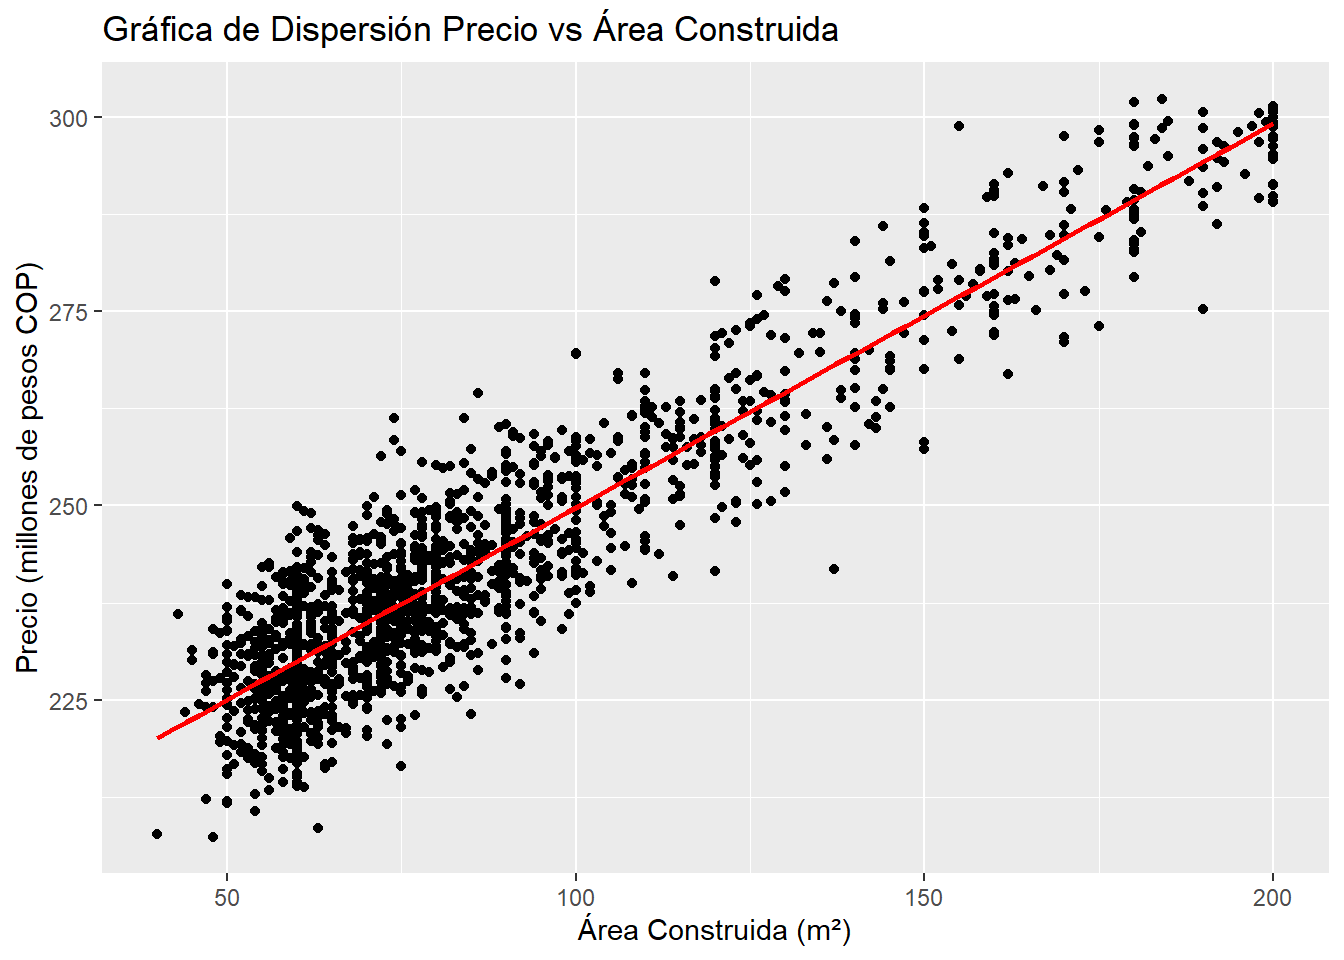
\includegraphics{Activdad_03_files/figure-latex/unnamed-chunk-16-1.pdf}

\subsubsection{1.1 Análisis para
Apartamentos}\label{anuxe1lisis-para-apartamentos}

\begin{Shaded}
\begin{Highlighting}[]
\NormalTok{aptos }\OtherTok{\textless{}{-}} \FunctionTok{subset}\NormalTok{(vivienda4, vivienda4}\SpecialCharTok{$}\NormalTok{tipo }\SpecialCharTok{==} \StringTok{"Apartamento"}\NormalTok{)}
\FunctionTok{summary}\NormalTok{(aptos)}
\end{Highlighting}
\end{Shaded}

\begin{verbatim}
##            zona      estrato     preciom        areaconst    
##  Zona Centro :   7   3:   0   Min.   :207.4   Min.   : 40.0  
##  Zona Norte  : 236   4:1361   1st Qu.:228.8   1st Qu.: 60.0  
##  Zona Oeste  :  52   5:   0   Median :236.1   Median : 70.0  
##  Zona Oriente:   2   6:   0   Mean   :237.6   Mean   : 75.3  
##  Zona Sur    :1064            3rd Qu.:243.6   3rd Qu.: 83.0  
##                               Max.   :300.6   Max.   :200.0  
##           tipo     
##  Apartamento:1361  
##  Casa       :   0  
##                    
##                    
##                    
## 
\end{verbatim}

Como podemos apreciar al ver el resumen del dataframe para los
apartamentos, se destaca lo siguiente: - Los apartamentos de estrato 4
tienen un rango de precios que va desde \$207.4 millones hasta \$300.6
millones, con un precio promedio de \$237.6 millones. - El 50\% de estos
apartamentos se encuentran en un rango de precios entre \$228.8 y
\$243.6 millones. - Un 25\% de los apartamentos tiene un precio inferior
a \$228.8 millones, mientras que el otro 25\% restante supera los
\$243.6 millones. - En cuanto al área construida, las propiedades varían
desde 40 m² hasta un máximo de 200 m², con un promedio de 75.3 m². La
mitad de los apartamentos tiene un área construida que oscila entre 60
m² y 83 m². El 25\% tiene menos de 60 m² y el 25\% supera los 83 m².

\begin{Shaded}
\begin{Highlighting}[]
\CommentTok{\# Validar si existen valores atípicos en los apartamentos}
\FunctionTok{par}\NormalTok{(}\AttributeTok{mfrow =} \FunctionTok{c}\NormalTok{(}\DecValTok{1}\NormalTok{, }\DecValTok{2}\NormalTok{))}
\FunctionTok{boxplot}\NormalTok{(aptos}\SpecialCharTok{$}\NormalTok{preciom, }\AttributeTok{main =} \StringTok{"Precio de apartamentos"}\NormalTok{, }\AttributeTok{col =} \StringTok{"cyan"}\NormalTok{)}
\FunctionTok{boxplot}\NormalTok{(aptos}\SpecialCharTok{$}\NormalTok{areaconst, }\AttributeTok{main =} \StringTok{"Área construida de apartamentos"}\NormalTok{, }\AttributeTok{col =}\StringTok{"green"}\NormalTok{)}
\end{Highlighting}
\end{Shaded}

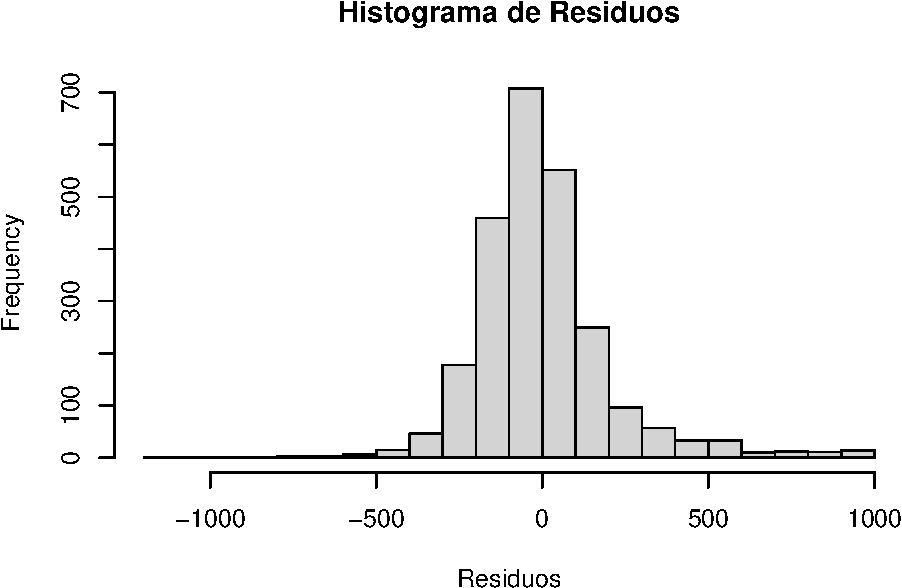
\includegraphics{Activdad_03_files/figure-latex/unnamed-chunk-18-1.pdf}

\begin{Shaded}
\begin{Highlighting}[]
\FunctionTok{par}\NormalTok{(}\AttributeTok{mfrow =} \FunctionTok{c}\NormalTok{(}\DecValTok{1}\NormalTok{, }\DecValTok{1}\NormalTok{))}
\end{Highlighting}
\end{Shaded}

Como se aprecia en el gráfico anterior, tanto el precio como el área
construida muestran la presencia de valores atípicos, ya que hay puntos
extremos (bigotes) que sobresalen por encima de la caja. Además, los
precios presentan un nivel de simetría, dado que los datos están
distribuidos de manera equilibrada alrededor de la mediana.

En cuanto al área construida, se observa una ligera asimetría en los
datos, con un sesgo leve hacia la parte inferior.

\begin{Shaded}
\begin{Highlighting}[]
\FunctionTok{par}\NormalTok{(}\AttributeTok{mfrow =} \FunctionTok{c}\NormalTok{(}\DecValTok{1}\NormalTok{, }\DecValTok{2}\NormalTok{))}

\CommentTok{\# Histograma del precio}
\FunctionTok{hist}\NormalTok{(aptos}\SpecialCharTok{$}\NormalTok{preciom, }\AttributeTok{main =} \StringTok{"Histograma de precio"}\NormalTok{, }\AttributeTok{xlab =} \StringTok{"Precio"}\NormalTok{, }\AttributeTok{col =} \StringTok{"cyan"}\NormalTok{)}

\CommentTok{\# Histograma del área construida}
\FunctionTok{hist}\NormalTok{(aptos}\SpecialCharTok{$}\NormalTok{areaconst, }\AttributeTok{main =} \StringTok{"Histograma de área construida"}\NormalTok{, }\AttributeTok{xlab =} \StringTok{"Área construida"}\NormalTok{, }\AttributeTok{col =}\StringTok{"green"}\NormalTok{)}
\end{Highlighting}
\end{Shaded}

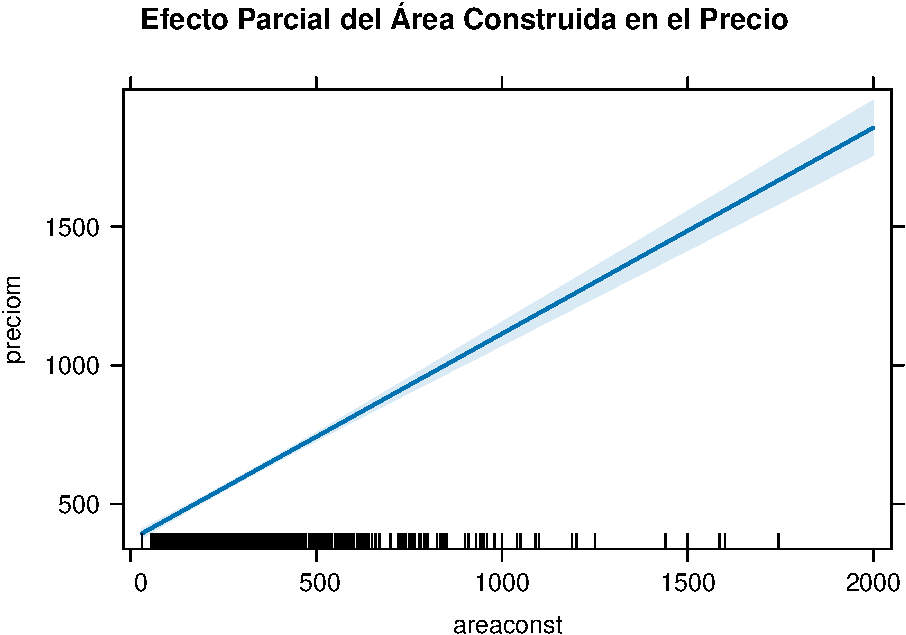
\includegraphics{Activdad_03_files/figure-latex/unnamed-chunk-19-1.pdf}

Como se puede apreciar, ambos histogramas revelan que los datos tanto
del precio como del área construida presentan una distribución no
normal, con un sesgo hacia la derecha.

Para corroborar esta no normalidad, se aplicó la prueba estadística de
Shapiro-Wilk a ambas variables.

\begin{Shaded}
\begin{Highlighting}[]
\FunctionTok{library}\NormalTok{(stats)}
\FunctionTok{shapiro.test}\NormalTok{(aptos}\SpecialCharTok{$}\NormalTok{preciom)}
\end{Highlighting}
\end{Shaded}

\begin{verbatim}
## 
##  Shapiro-Wilk normality test
## 
## data:  aptos$preciom
## W = 0.93585, p-value < 2.2e-16
\end{verbatim}

\begin{Shaded}
\begin{Highlighting}[]
\FunctionTok{shapiro.test}\NormalTok{(aptos}\SpecialCharTok{$}\NormalTok{areaconst)}
\end{Highlighting}
\end{Shaded}

\begin{verbatim}
## 
##  Shapiro-Wilk normality test
## 
## data:  aptos$areaconst
## W = 0.83373, p-value < 2.2e-16
\end{verbatim}

De lo anterior, es posible verficar que los p-valores son menores a
0.05, por lo cual, la hipótesis nula se rechaza y confirmando que las
dos variables sigue una distribución normal.

\subsubsection{1.2 Análisis para
Apartamentos}\label{anuxe1lisis-para-apartamentos-1}

\begin{Shaded}
\begin{Highlighting}[]
\NormalTok{casas }\OtherTok{\textless{}{-}} \FunctionTok{subset}\NormalTok{(vivienda4, vivienda4}\SpecialCharTok{$}\NormalTok{tipo }\SpecialCharTok{==} \StringTok{"Casa"}\NormalTok{)}
\FunctionTok{summary}\NormalTok{(casas)}
\end{Highlighting}
\end{Shaded}

\begin{verbatim}
##            zona     estrato    preciom        areaconst              tipo    
##  Zona Centro :  1   3:  0   Min.   :221.3   Min.   : 54.0   Apartamento:  0  
##  Zona Norte  : 48   4:326   1st Qu.:250.4   1st Qu.:100.0   Casa       :326  
##  Zona Oeste  :  8   5:  0   Median :263.5   Median :127.5                    
##  Zona Oriente:  4   6:  0   Mean   :265.7   Mean   :132.8                    
##  Zona Sur    :265           3rd Qu.:284.1   3rd Qu.:164.8                    
##                             Max.   :302.3   Max.   :200.0
\end{verbatim}

Por el lado de las casas, al ver el resumen del dataframe se destaca lo
siguiente:

\begin{itemize}
\item
  Las casas son de estrato 4 y presentan precios que varían entre 221.3
  millones y 302.3 millones, con un promedio de 265.7 millones.
\item
  El 50\% de las casas tiene precios que oscilan entre 250.4 y 284.1
  millones, mientras que un 25\% cuesta menos de 250.4 millones y el
  otro 25\% supera los 284.1 millones.
\item
  En cuanto al área construida, las casas van desde 54 m² hasta 200 m²,
  con una media de 135.9 m². - La mitad de las casas tiene un área
  construida que oscila entre 100 y 170 m².
\item
  Un 25\% de las casas tiene menos de 100 m², mientras que otro 25\%
  supera los 170 m².
\end{itemize}

\begin{Shaded}
\begin{Highlighting}[]
\FunctionTok{par}\NormalTok{(}\AttributeTok{mfrow =} \FunctionTok{c}\NormalTok{(}\DecValTok{1}\NormalTok{, }\DecValTok{2}\NormalTok{))}
\FunctionTok{boxplot}\NormalTok{(casas}\SpecialCharTok{$}\NormalTok{preciom, }\AttributeTok{main =} \StringTok{"Precio de casas"}\NormalTok{, }\AttributeTok{col =} \StringTok{"\#54FF9F"}\NormalTok{)}
\FunctionTok{boxplot}\NormalTok{(casas}\SpecialCharTok{$}\NormalTok{areaconst, }\AttributeTok{main =} \StringTok{"Área construida de casas"}\NormalTok{, }\AttributeTok{col =}\StringTok{"\#F0E68C"}\NormalTok{)}
\end{Highlighting}
\end{Shaded}

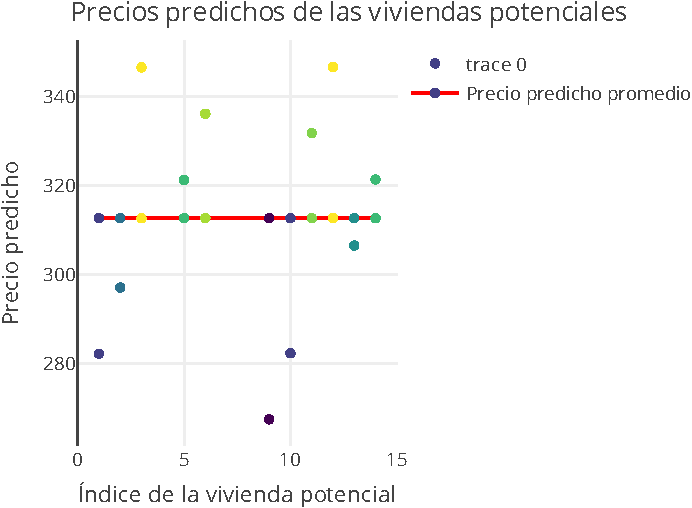
\includegraphics{Activdad_03_files/figure-latex/unnamed-chunk-22-1.pdf}

\begin{Shaded}
\begin{Highlighting}[]
\FunctionTok{par}\NormalTok{(}\AttributeTok{mfrow =} \FunctionTok{c}\NormalTok{(}\DecValTok{1}\NormalTok{, }\DecValTok{1}\NormalTok{))}
\end{Highlighting}
\end{Shaded}

Como se puede observar en el gráfico de cajas anterior, tanto el precio
como el área construida muestran una cierta simetría en sus datos, sin
evidencia de valores atípicos.

\begin{Shaded}
\begin{Highlighting}[]
\FunctionTok{par}\NormalTok{(}\AttributeTok{mfrow =} \FunctionTok{c}\NormalTok{(}\DecValTok{1}\NormalTok{, }\DecValTok{2}\NormalTok{))}
\FunctionTok{hist}\NormalTok{(casas}\SpecialCharTok{$}\NormalTok{preciom, }\AttributeTok{main =} \StringTok{"Histograma de precio"}\NormalTok{, }\AttributeTok{xlab =} \StringTok{"Precio"}\NormalTok{, }\AttributeTok{col =} \StringTok{"\#54FF9F"}\NormalTok{)}
\FunctionTok{hist}\NormalTok{(casas}\SpecialCharTok{$}\NormalTok{areaconst, }\AttributeTok{main =} \StringTok{"Histograma de área construida"}\NormalTok{, }\AttributeTok{xlab =} \StringTok{"Área construida"}\NormalTok{, }\AttributeTok{col =}\StringTok{"\#F0E68C"}\NormalTok{)}
\end{Highlighting}
\end{Shaded}

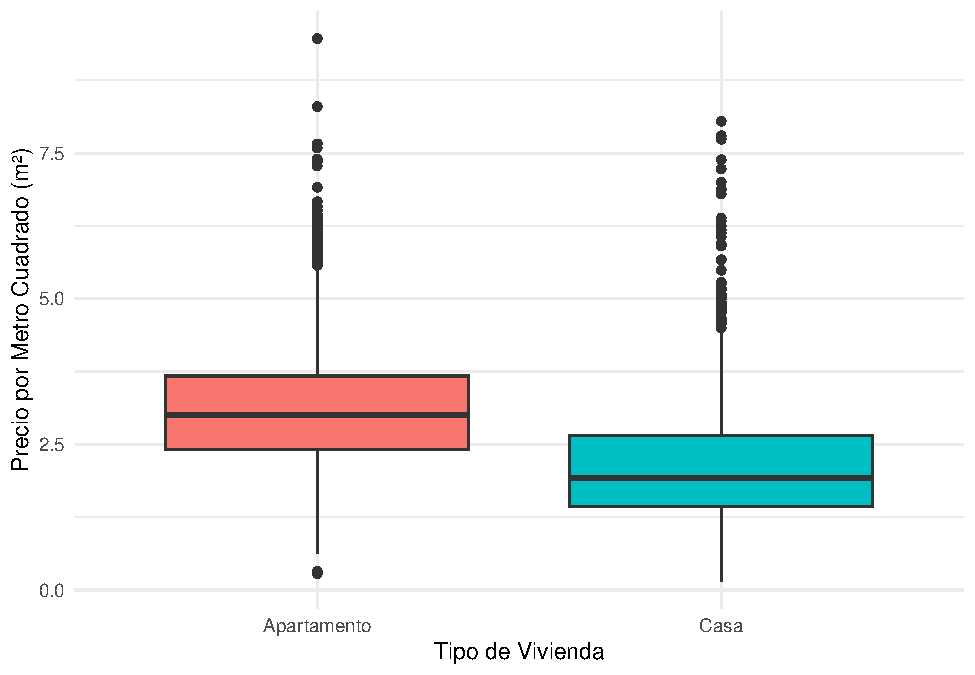
\includegraphics{Activdad_03_files/figure-latex/unnamed-chunk-23-1.pdf}

\begin{Shaded}
\begin{Highlighting}[]
\FunctionTok{par}\NormalTok{(}\AttributeTok{mfrow =} \FunctionTok{c}\NormalTok{(}\DecValTok{1}\NormalTok{, }\DecValTok{1}\NormalTok{))}
\end{Highlighting}
\end{Shaded}

No obstante, el histograma revela que los datos no siguen una
distribución normal para ambas variables. Para confirmar esta no
normalidad, se aplica la prueba estadística de Shapiro-Wilk.

\begin{Shaded}
\begin{Highlighting}[]
\FunctionTok{shapiro.test}\NormalTok{(casas}\SpecialCharTok{$}\NormalTok{preciom)}
\end{Highlighting}
\end{Shaded}

\begin{verbatim}
## 
##  Shapiro-Wilk normality test
## 
## data:  casas$preciom
## W = 0.9691, p-value = 1.966e-06
\end{verbatim}

\begin{Shaded}
\begin{Highlighting}[]
\FunctionTok{shapiro.test}\NormalTok{(casas}\SpecialCharTok{$}\NormalTok{areaconst)}
\end{Highlighting}
\end{Shaded}

\begin{verbatim}
## 
##  Shapiro-Wilk normality test
## 
## data:  casas$areaconst
## W = 0.96244, p-value = 1.934e-07
\end{verbatim}

El test anterior muestra p-valores menores a 0.05. lo que permite
rechazar la hipótesis nula, afirmando así que ninguna de las dos
variables presenta una distribución normal.

\section{\texorpdfstring{\textbf{2. Realice un análisis exploratorio
bivariado de datos, enfocado en la relación entre la variable respuesta
(precio) en función de la variable predictora (area construida) -
incluir gráficos e indicadores apropiados
interpretados.}}{2. Realice un análisis exploratorio bivariado de datos, enfocado en la relación entre la variable respuesta (precio) en función de la variable predictora (area construida) - incluir gráficos e indicadores apropiados interpretados.}}\label{realice-un-anuxe1lisis-exploratorio-bivariado-de-datos-enfocado-en-la-relaciuxf3n-entre-la-variable-respuesta-precio-en-funciuxf3n-de-la-variable-predictora-area-construida---incluir-gruxe1ficos-e-indicadores-apropiados-interpretados.}

\begin{Shaded}
\begin{Highlighting}[]
\CommentTok{\# Gráfico de dispersión (precio vs área construida) con línea de tendencia central}
\FunctionTok{ggplot}\NormalTok{(vivienda4, }\FunctionTok{aes}\NormalTok{(}\AttributeTok{x =}\NormalTok{ areaconst, }\AttributeTok{y =}\NormalTok{ preciom)) }\SpecialCharTok{+}
  \FunctionTok{geom\_point}\NormalTok{() }\SpecialCharTok{+}
  \FunctionTok{geom\_smooth}\NormalTok{(}\AttributeTok{method =} \StringTok{"lm"}\NormalTok{, }\AttributeTok{color =} \StringTok{"red"}\NormalTok{, }\AttributeTok{se =} \ConstantTok{FALSE}\NormalTok{) }\SpecialCharTok{+}  \CommentTok{\# Línea de tendencia}
  \FunctionTok{labs}\NormalTok{(}\AttributeTok{x =} \StringTok{"Área Construida (m²)"}\NormalTok{, }\AttributeTok{y =} \StringTok{"Precio (millones de pesos COP)"}\NormalTok{) }\SpecialCharTok{+}
  \FunctionTok{ggtitle}\NormalTok{(}\StringTok{"Gráfico de Dispersión Precio vs Área Construida"}\NormalTok{)}
\end{Highlighting}
\end{Shaded}

\begin{verbatim}
## `geom_smooth()` using formula = 'y ~ x'
\end{verbatim}

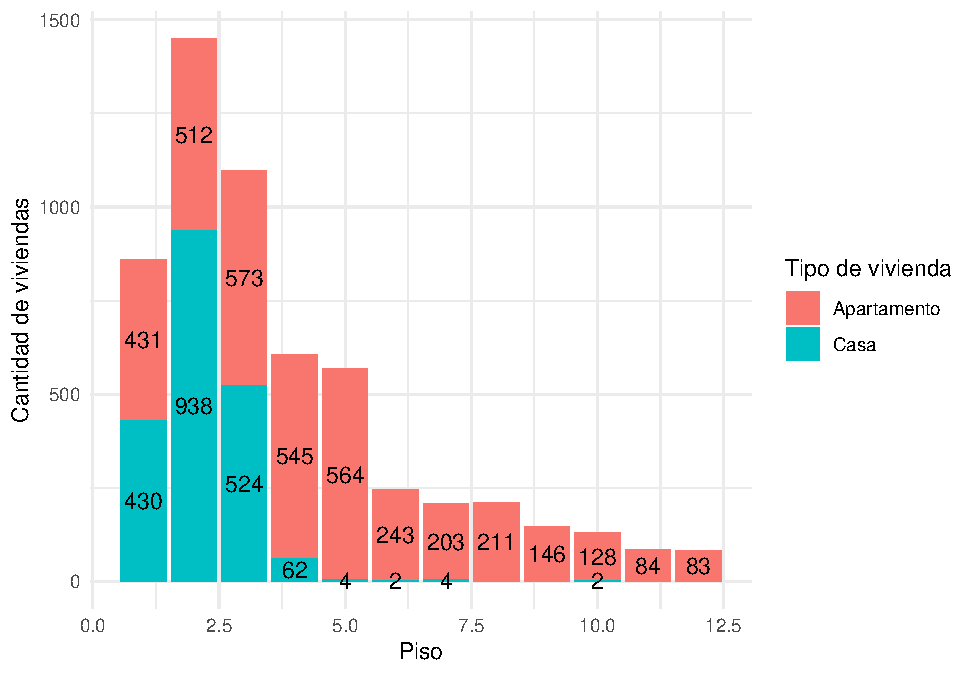
\includegraphics{Activdad_03_files/figure-latex/unnamed-chunk-25-1.pdf}

El gráfico de dispersión sugiere una relación lineal entre las dos
variables, mostrando que a medida que aumenta el área construida,
también lo hace el precio de los apartamentos. Para confirmar esta
relación positiva, se aplicaremos la prueba no paramétrica de Spearman,
debido a la distribución no normal de los datos.

\begin{Shaded}
\begin{Highlighting}[]
\FunctionTok{cor.test}\NormalTok{(aptos}\SpecialCharTok{$}\NormalTok{areaconst, aptos}\SpecialCharTok{$}\NormalTok{preciom)}
\end{Highlighting}
\end{Shaded}

\begin{verbatim}
## 
##  Pearson's product-moment correlation
## 
## data:  aptos$areaconst and aptos$preciom
## t = 57.087, df = 1359, p-value < 2.2e-16
## alternative hypothesis: true correlation is not equal to 0
## 95 percent confidence interval:
##  0.8236972 0.8550345
## sample estimates:
##       cor 
## 0.8400653
\end{verbatim}

\begin{Shaded}
\begin{Highlighting}[]
\FunctionTok{cor.test}\NormalTok{(aptos}\SpecialCharTok{$}\NormalTok{areaconst, aptos}\SpecialCharTok{$}\NormalTok{preciom, }\AttributeTok{method =} \StringTok{"spearman"}\NormalTok{)}
\end{Highlighting}
\end{Shaded}

\begin{verbatim}
## Warning in cor.test.default(aptos$areaconst, aptos$preciom, method =
## "spearman"): Cannot compute exact p-value with ties
\end{verbatim}

\begin{verbatim}
## 
##  Spearman's rank correlation rho
## 
## data:  aptos$areaconst and aptos$preciom
## S = 109350726, p-value < 2.2e-16
## alternative hypothesis: true rho is not equal to 0
## sample estimates:
##       rho 
## 0.7397452
\end{verbatim}

Con base en lo anterior, el test de Pearson arroja una correlación
positiva de 0.83, mientras que la prueba no paramétrica de Spearman
muestra un coeficiente de 0.738. De esto, podemos inferir que:

\begin{itemize}
\tightlist
\item
  Ambos resultados confirman una correlación positiva con un buen
  ajuste, siendo estadísticamente significativa con un p-value
  \textless{} 2.2e-16.
\item
  Este resultado indica una elasticidad unitaria entre las variables,
  dado que a medida que aumenta el área construida, también aumenta el
  precio, y esta relación es muy fuerte, como lo evidencia el valor
  pequeño del p-value .
\end{itemize}

\section{\texorpdfstring{\textbf{3. Estime el modelo de regresión lineal
simple entre precio=f(area)+ε. Interprete los coeficientes del modelo
β0, β1 en caso de ser
correcto.}}{3. Estime el modelo de regresión lineal simple entre precio=f(area)+ε. Interprete los coeficientes del modelo β0, β1 en caso de ser correcto.}}\label{estime-el-modelo-de-regresiuxf3n-lineal-simple-entre-preciofareaux3b5.-interprete-los-coeficientes-del-modelo-ux3b20-ux3b21-en-caso-de-ser-correcto.}

\begin{Shaded}
\begin{Highlighting}[]
\CommentTok{\# Estimar el modelo de regresión lineal simple}
\CommentTok{\#modelo\_regresion \textless{}{-} lm(preciom \textasciitilde{} areaconst, data = vivienda4)}

\CommentTok{\# Mostrar un resumen del modelo}
\CommentTok{\#summary(modelo\_regresion)}
\end{Highlighting}
\end{Shaded}

\paragraph{\texorpdfstring{\textbf{Para los
apartamentos}}{Para los apartamentos}}\label{para-los-apartamentos}

\begin{Shaded}
\begin{Highlighting}[]
\NormalTok{modelo\_regresion1 }\OtherTok{\textless{}{-}} \FunctionTok{lm}\NormalTok{(aptos}\SpecialCharTok{$}\NormalTok{preciom}\SpecialCharTok{\textasciitilde{}}\NormalTok{aptos}\SpecialCharTok{$}\NormalTok{areaconst)}
\NormalTok{resultado\_prueba1 }\OtherTok{\textless{}{-}} \FunctionTok{summary}\NormalTok{(modelo\_regresion1)}
\NormalTok{resultado\_prueba1}
\end{Highlighting}
\end{Shaded}

\begin{verbatim}
## 
## Call:
## lm(formula = aptos$preciom ~ aptos$areaconst)
## 
## Residuals:
##      Min       1Q   Median       3Q      Max 
## -26.4137  -5.0770  -0.0061   4.6197  24.3348 
## 
## Coefficients:
##                  Estimate Std. Error t value Pr(>|t|)    
## (Intercept)     2.002e+02  6.829e-01  293.11   <2e-16 ***
## aptos$areaconst 4.969e-01  8.704e-03   57.09   <2e-16 ***
## ---
## Signif. codes:  0 '***' 0.001 '**' 0.01 '*' 0.05 '.' 0.1 ' ' 1
## 
## Residual standard error: 7.084 on 1359 degrees of freedom
## Multiple R-squared:  0.7057, Adjusted R-squared:  0.7055 
## F-statistic:  3259 on 1 and 1359 DF,  p-value: < 2.2e-16
\end{verbatim}

\begin{Shaded}
\begin{Highlighting}[]
\CommentTok{\# Mostrar un resumen del modelo}
\FunctionTok{summary}\NormalTok{(resultado\_prueba1)}
\end{Highlighting}
\end{Shaded}

\begin{verbatim}
##               Length Class  Mode   
## call             2   -none- call   
## terms            3   terms  call   
## residuals     1361   -none- numeric
## coefficients     8   -none- numeric
## aliased          2   -none- logical
## sigma            1   -none- numeric
## df               3   -none- numeric
## r.squared        1   -none- numeric
## adj.r.squared    1   -none- numeric
## fstatistic       3   -none- numeric
## cov.unscaled     4   -none- numeric
\end{verbatim}

El coeficiente del intercepto (β0) en el modelo de regresión lineal es
de 200.2 millones de pesos COP. Sin embargo, su interpretación en este
contexto puede carecer de significado práctico, porque este valor hace
referencia al precio estimado cuando el área construida es igual a cero,
lo cual no tiene una interpretación realista en el contexto de bienes
raíces.

Por otro lado, el coeficiente de la variable ``areaconst'' (β1) es de
0.4962, lo que significa que por cada metro cuadrado adicional de área
construida, se espera un incremento promedio en el precio de 0.4962
millones de pesos COP, es decir, que el precio promedio de una vivienda
de tipo apartamento aumenta en aproximadamente 0.4962 millones de pesos
COP por cada metro cuadrado adicional de área construida.

\paragraph{\texorpdfstring{\textbf{Para las
casas}}{Para las casas}}\label{para-las-casas}

\begin{Shaded}
\begin{Highlighting}[]
\NormalTok{modelo\_regresionCasas }\OtherTok{=} \FunctionTok{lm}\NormalTok{ (preciom }\SpecialCharTok{\textasciitilde{}}\NormalTok{ areaconst, casas)}
\FunctionTok{summary}\NormalTok{(modelo\_regresionCasas)}
\end{Highlighting}
\end{Shaded}

\begin{verbatim}
## 
## Call:
## lm(formula = preciom ~ areaconst, data = casas)
## 
## Residuals:
##      Min       1Q   Median       3Q      Max 
## -18.9715  -4.4788  -0.2916   4.4190  21.9460 
## 
## Coefficients:
##              Estimate Std. Error t value Pr(>|t|)    
## (Intercept) 199.29486    1.44773  137.66   <2e-16 ***
## areaconst     0.49991    0.01047   47.76   <2e-16 ***
## ---
## Signif. codes:  0 '***' 0.001 '**' 0.01 '*' 0.05 '.' 0.1 ' ' 1
## 
## Residual standard error: 7.341 on 324 degrees of freedom
## Multiple R-squared:  0.8756, Adjusted R-squared:  0.8753 
## F-statistic:  2281 on 1 and 324 DF,  p-value: < 2.2e-16
\end{verbatim}

Para este caso, el coeficiente del intercepto β0 es de 200.19, lo que
indica el precio del terreno sin área construida en millones de pesos
COP. Además, el coeficiente R2 tiene un valor de 0.8659, lo que
significa que el modelo cuenta con un 87\% aprox. de la variación del
precio, teniendo en cuenta el área de la casa.

Por el lado de la pendiente β1, presenta un valor de 0.49093, indicando
que por cada aumento de un metro cuadrado de las casas el precio se
incrementa en 0.49093 Millones. Adicionalmente, el valor de P es de
\textless2e-16, lo que nos indica su significancia.

\section{\texorpdfstring{\textbf{4. Construir un intervalo de confianza
(95\%) para el coeficiente β1, interpretar y concluir si el coeficiente
es igual a cero o no. Compare este resultado con una prueba de hipótesis
t.}}{4. Construir un intervalo de confianza (95\%) para el coeficiente β1, interpretar y concluir si el coeficiente es igual a cero o no. Compare este resultado con una prueba de hipótesis t.}}\label{construir-un-intervalo-de-confianza-95-para-el-coeficiente-ux3b21-interpretar-y-concluir-si-el-coeficiente-es-igual-a-cero-o-no.-compare-este-resultado-con-una-prueba-de-hipuxf3tesis-t.}

\paragraph{Análisis para los
apartamentos}\label{anuxe1lisis-para-los-apartamentos}

\begin{Shaded}
\begin{Highlighting}[]
\CommentTok{\#intervalo\_confianza \textless{}{-}confint(modelo\_regresion1, level = 0.95)}
\CommentTok{\#intervalo\_confianza}
\end{Highlighting}
\end{Shaded}

\begin{Shaded}
\begin{Highlighting}[]
\CommentTok{\# Obtener el valor crítico de la distribución t}
\NormalTok{grados\_libertadAptos }\OtherTok{\textless{}{-}} \FunctionTok{length}\NormalTok{(aptos}\SpecialCharTok{$}\NormalTok{areaconst) }\SpecialCharTok{{-}} \DecValTok{2}
\NormalTok{t\_criticoAptos }\OtherTok{\textless{}{-}} \FunctionTok{qt}\NormalTok{(}\FloatTok{0.975}\NormalTok{, }\AttributeTok{df =}\NormalTok{ grados\_libertadAptos)  }\CommentTok{\# Para un intervalo de confianza del 95\%}

\CommentTok{\# Calcular el intervalo de confianza para β1}
\NormalTok{coef\_beta1Aptos }\OtherTok{\textless{}{-}} \FunctionTok{coef}\NormalTok{(modelo\_regresion1)[}\DecValTok{2}\NormalTok{]  }\CommentTok{\# Coeficiente β1}
\NormalTok{se\_beta1Aptos }\OtherTok{\textless{}{-}} \FunctionTok{summary}\NormalTok{(modelo\_regresion1)}\SpecialCharTok{$}\NormalTok{coefficients[}\DecValTok{2}\NormalTok{, }\StringTok{"Std. Error"}\NormalTok{]  }\CommentTok{\# Error estándar de β1}

\NormalTok{limite\_inferiorAptos }\OtherTok{\textless{}{-}}\NormalTok{ coef\_beta1Aptos }\SpecialCharTok{{-}}\NormalTok{ t\_criticoAptos }\SpecialCharTok{*}\NormalTok{ se\_beta1Aptos}
\NormalTok{limite\_superiorAptos }\OtherTok{\textless{}{-}}\NormalTok{ coef\_beta1Aptos }\SpecialCharTok{+}\NormalTok{ t\_criticoAptos }\SpecialCharTok{*}\NormalTok{ se\_beta1Aptos}

\CommentTok{\# Mostrar el intervalo de confianza}
\FunctionTok{cat}\NormalTok{(}\StringTok{"Intervalo de Confianza (95\%) para β1: ["}\NormalTok{, limite\_inferiorAptos, }\StringTok{", "}\NormalTok{, limite\_superiorAptos, }\StringTok{"]}\SpecialCharTok{\textbackslash{}n}\StringTok{Valor β1:"}\NormalTok{, coef\_beta1Aptos)}
\end{Highlighting}
\end{Shaded}

\begin{verbatim}
## Intervalo de Confianza (95%) para β1: [ 0.4798137 ,  0.5139636 ]
## Valor β1: 0.4968887
\end{verbatim}

\begin{Shaded}
\begin{Highlighting}[]
\CommentTok{\# Realizar la prueba de hipótesis t}
\NormalTok{t\_statAptos }\OtherTok{\textless{}{-}}\NormalTok{ coef\_beta1Aptos }\SpecialCharTok{/}\NormalTok{ se\_beta1Aptos}
\NormalTok{grados\_libertadAptos }\OtherTok{\textless{}{-}} \FunctionTok{length}\NormalTok{(aptos}\SpecialCharTok{$}\NormalTok{areaconst) }\SpecialCharTok{{-}} \DecValTok{2}
\NormalTok{p\_valor }\OtherTok{\textless{}{-}} \DecValTok{2} \SpecialCharTok{*}\NormalTok{ (}\DecValTok{1} \SpecialCharTok{{-}} \FunctionTok{pt}\NormalTok{(}\FunctionTok{abs}\NormalTok{(t\_statAptos), }\AttributeTok{df =}\NormalTok{ grados\_libertadAptos))}

\CommentTok{\# Mostrar el estadístico t y el p{-}valor}
\FunctionTok{cat}\NormalTok{(}\StringTok{"Estadístico t para β1:"}\NormalTok{, t\_statAptos, }\StringTok{"}\SpecialCharTok{\textbackslash{}n}\StringTok{"}\NormalTok{)}
\end{Highlighting}
\end{Shaded}

\begin{verbatim}
## Estadístico t para β1: 57.08668
\end{verbatim}

Determinando el intervalo de confianza del 95\%, se puede inferir que el
coeficiente β1 se encuentra dentro de este intervalo, lo que sugiere que
por cada metro cuadrado adicional en el apartamento, el valor promedio
de la variable endógena, el precio, aumentaría entre 0.47 y 0.51
millones de pesos COP. Además, el hecho de que el intervalo no contenga
el valor cero indica que el coeficiente β1 es diferente de cero, lo que
sugiere una relación significativa entre el precio y el área construida.

Para verificar este resultado mediante una prueba de hipótesis, se
utiliza la prueba t para β1, con el objetivo de determinar si el
coeficiente es igual a cero (hipótesis nula) o no (hipótesis
alternativa).

\begin{Shaded}
\begin{Highlighting}[]
\FunctionTok{cat}\NormalTok{(}\StringTok{"P{-}valor de la prueba de hipótesis t:"}\NormalTok{, p\_valor, }\StringTok{"}\SpecialCharTok{\textbackslash{}n}\StringTok{"}\NormalTok{)}
\end{Highlighting}
\end{Shaded}

\begin{verbatim}
## P-valor de la prueba de hipótesis t: 0
\end{verbatim}

\begin{Shaded}
\begin{Highlighting}[]
\CommentTok{\#valor\_p \textless{}{-} resultado\_prueba1$coefficients["aptos$areaconst", "Pr(\textgreater{}|t|)"]}
\CommentTok{\#valor\_p}
\end{Highlighting}
\end{Shaded}

Dado que el p-valor es extremadamente bajo, (cero), y menor que el nivel
de significancia, se rechaza la hipótesis nula que planteaba que el
coeficiente β1 es igual a cero.

Esto indica que el coeficiente β1 es significativamente diferente de
cero, lo que confirma la existencia de una relación lineal significativa
entre los metros cuadrados de los apartamentos y su precio. El
estadístico t, que es 54.95302, refuerza esta conclusión, proporcionando
evidencia estadística sólida de que el área construida contribuye de
manera importante a explicar las variaciones en el precio de los
apartamentos.

Se puede concluir que, tanto el intervalo de confianza como la prueba de
hipótesis t confirman que el coeficiente β1 es significativamente
diferente de cero, respaldando así la afirmación sobre el impacto
considerable que tiene el área construida en el precio de los
apartamentos.

\paragraph{Análisis para las casas}\label{anuxe1lisis-para-las-casas}

\begin{Shaded}
\begin{Highlighting}[]
\CommentTok{\#intervalo\_confianza \textless{}{-}confint(modelo\_regresionCasas, level = 0.95)}
\CommentTok{\#intervalo\_confianza}
\end{Highlighting}
\end{Shaded}

\begin{Shaded}
\begin{Highlighting}[]
\CommentTok{\# Obtener el valor crítico de la distribución t}
\NormalTok{grados\_libertadCasas }\OtherTok{\textless{}{-}} \FunctionTok{length}\NormalTok{(casas}\SpecialCharTok{$}\NormalTok{areaconst) }\SpecialCharTok{{-}} \DecValTok{2}
\NormalTok{t\_criticoCasas }\OtherTok{\textless{}{-}} \FunctionTok{qt}\NormalTok{(}\FloatTok{0.975}\NormalTok{, }\AttributeTok{df =}\NormalTok{ grados\_libertadCasas)  }\CommentTok{\# Para un intervalo de confianza del 95\%}

\CommentTok{\# Calcular el intervalo de confianza para β1}
\NormalTok{coef\_beta1Casas }\OtherTok{\textless{}{-}} \FunctionTok{coef}\NormalTok{(modelo\_regresionCasas)[}\DecValTok{2}\NormalTok{]  }\CommentTok{\# Coeficiente β1}
\NormalTok{se\_beta1Casas }\OtherTok{\textless{}{-}} \FunctionTok{summary}\NormalTok{(modelo\_regresionCasas)}\SpecialCharTok{$}\NormalTok{coefficients[}\DecValTok{2}\NormalTok{, }\StringTok{"Std. Error"}\NormalTok{]  }\CommentTok{\# Error estándar de β1}

\NormalTok{limite\_inferiorCasas }\OtherTok{\textless{}{-}}\NormalTok{ coef\_beta1Casas }\SpecialCharTok{{-}}\NormalTok{ t\_criticoCasas }\SpecialCharTok{*}\NormalTok{ se\_beta1Casas}
\NormalTok{limite\_superiorCasas }\OtherTok{\textless{}{-}}\NormalTok{ coef\_beta1Casas }\SpecialCharTok{+}\NormalTok{ t\_criticoCasas }\SpecialCharTok{*}\NormalTok{ se\_beta1Casas}

\CommentTok{\# Mostrar el intervalo de confianza}
\FunctionTok{cat}\NormalTok{(}\StringTok{"Intervalo de Confianza (95\%) para β1: ["}\NormalTok{, limite\_inferiorCasas, }\StringTok{", "}\NormalTok{, limite\_superiorCasas, }\StringTok{"]}\SpecialCharTok{\textbackslash{}n}\StringTok{Valor β1:"}\NormalTok{, coef\_beta1Casas)}
\end{Highlighting}
\end{Shaded}

\begin{verbatim}
## Intervalo de Confianza (95%) para β1: [ 0.4793188 ,  0.5204997 ]
## Valor β1: 0.4999092
\end{verbatim}

De igual manera, con un nivel de confianza del 95\%, se puede concluir
que por cada metro cuadrado adicional que se incremente en la casa, el
precio podría aumentar entre 0.46 y 0.51 millones de pesos.

\begin{Shaded}
\begin{Highlighting}[]
\CommentTok{\# Gráfico del intervalo de confianza para β1}
\FunctionTok{library}\NormalTok{(ggplot2)}

\NormalTok{intervalo\_confianza }\OtherTok{\textless{}{-}} \FunctionTok{data.frame}\NormalTok{(}
  \AttributeTok{Intervalo =} \FunctionTok{c}\NormalTok{(}\StringTok{"Aptos"}\NormalTok{, }\StringTok{"Casas"}\NormalTok{), }
  \AttributeTok{Limite\_Inferior =} \FunctionTok{c}\NormalTok{(limite\_inferiorAptos, limite\_inferiorCasas), }
  \AttributeTok{Limite\_Superior =} \FunctionTok{c}\NormalTok{(limite\_superiorAptos, limite\_superiorCasas),}
  \AttributeTok{Estimado =} \FunctionTok{c}\NormalTok{(coef\_beta1Aptos, coef\_beta1Casas)}
\NormalTok{)}

\CommentTok{\# Crear el gráfico combinado para Aptos y Casas}
\FunctionTok{ggplot}\NormalTok{(intervalo\_confianza, }\FunctionTok{aes}\NormalTok{(}\AttributeTok{x =}\NormalTok{ Intervalo, }\AttributeTok{y =}\NormalTok{ Estimado, }\AttributeTok{color =}\NormalTok{ Intervalo)) }\SpecialCharTok{+}
  \FunctionTok{geom\_point}\NormalTok{(}\AttributeTok{size =} \DecValTok{3}\NormalTok{) }\SpecialCharTok{+}
  \FunctionTok{geom\_errorbar}\NormalTok{(}\FunctionTok{aes}\NormalTok{(}\AttributeTok{ymin =}\NormalTok{ Limite\_Inferior, }\AttributeTok{ymax =}\NormalTok{ Limite\_Superior), }\AttributeTok{width =} \FloatTok{0.2}\NormalTok{, }\AttributeTok{color =} \StringTok{"red"}\NormalTok{) }\SpecialCharTok{+}
  \FunctionTok{geom\_text}\NormalTok{(}\FunctionTok{aes}\NormalTok{(}\AttributeTok{label =} \FunctionTok{round}\NormalTok{(Estimado, }\DecValTok{3}\NormalTok{)), }\AttributeTok{vjust =} \SpecialCharTok{{-}}\DecValTok{1}\NormalTok{, }\AttributeTok{color =} \StringTok{"black"}\NormalTok{) }\SpecialCharTok{+}
  \FunctionTok{scale\_color\_manual}\NormalTok{(}\AttributeTok{values =} \FunctionTok{c}\NormalTok{(}\StringTok{"Aptos"} \OtherTok{=} \StringTok{"blue"}\NormalTok{, }\StringTok{"Casas"} \OtherTok{=} \StringTok{"green"}\NormalTok{)) }\SpecialCharTok{+}
  \FunctionTok{labs}\NormalTok{(}\AttributeTok{x =} \StringTok{""}\NormalTok{, }\AttributeTok{y =} \StringTok{"Coeficiente β1"}\NormalTok{) }\SpecialCharTok{+}
  \FunctionTok{ggtitle}\NormalTok{(}\StringTok{"Intervalos de Confianza (95\%) para β1: Aptos y Casas"}\NormalTok{) }\SpecialCharTok{+}
  \FunctionTok{theme\_minimal}\NormalTok{()}
\end{Highlighting}
\end{Shaded}

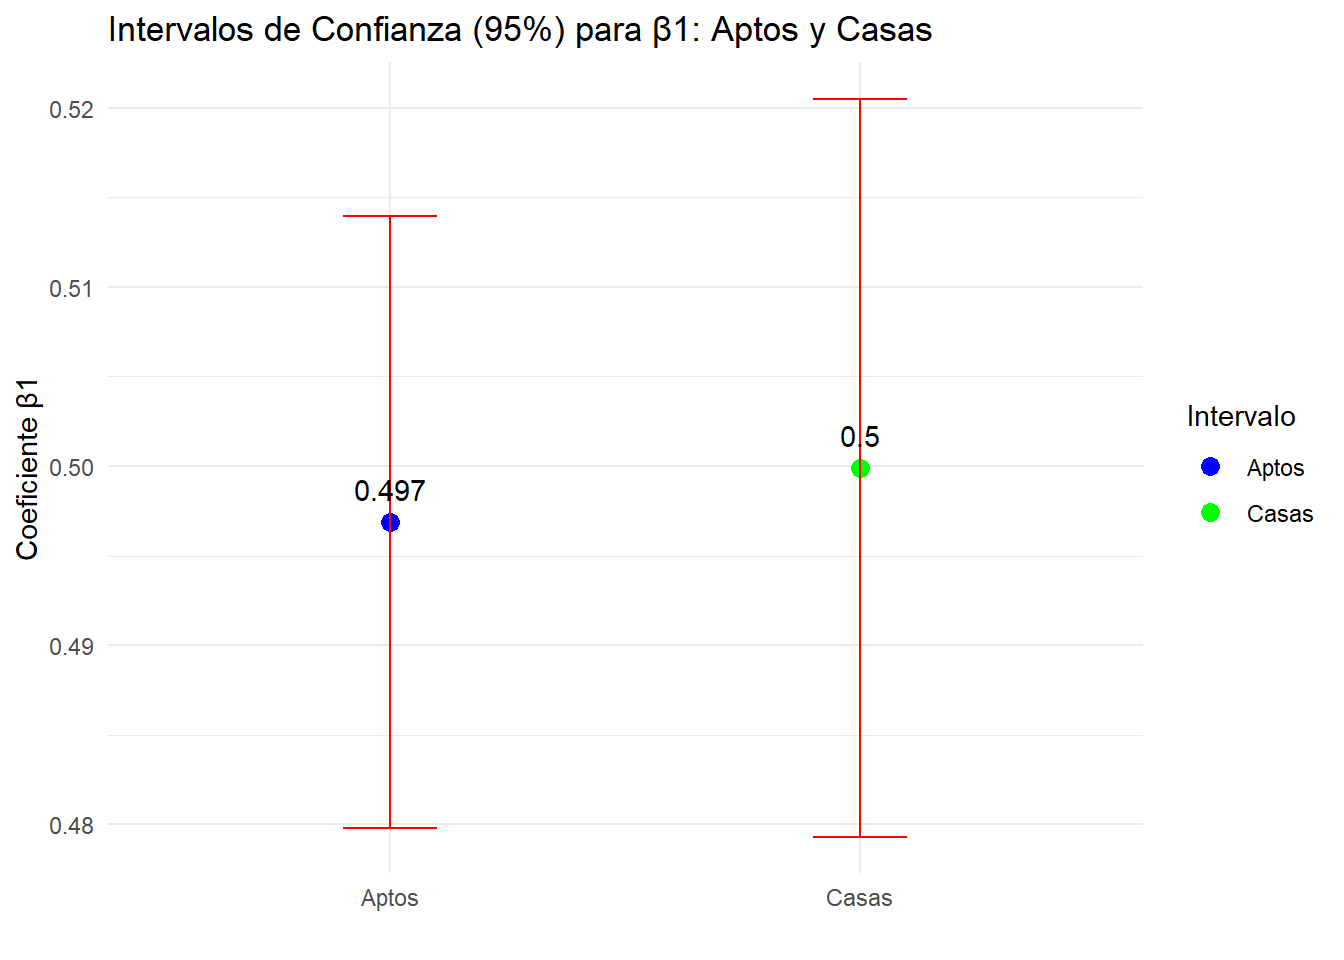
\includegraphics{Activdad_03_files/figure-latex/unnamed-chunk-37-1.pdf}

\section{\texorpdfstring{\textbf{5. Calcule e interprete el indicador de
bondad
R².}}{5. Calcule e interprete el indicador de bondad R².}}\label{calcule-e-interprete-el-indicador-de-bondad-ruxb2.}

\begin{Shaded}
\begin{Highlighting}[]
\NormalTok{R\_cuadrado }\OtherTok{\textless{}{-}} \FunctionTok{summary}\NormalTok{(modelo\_regresion1)}\SpecialCharTok{$}\NormalTok{r.squared}
\FunctionTok{cat}\NormalTok{(}\StringTok{"Coeficiente de Determinación (R²):"}\NormalTok{, R\_cuadrado, }\StringTok{"}\SpecialCharTok{\textbackslash{}n}\StringTok{"}\NormalTok{)}
\end{Highlighting}
\end{Shaded}

\begin{verbatim}
## Coeficiente de Determinación (R²): 0.7057097
\end{verbatim}

Sabemos que el coeficiente de determinación (R²) es un indicador
fundamental en análisis de regresión que mide la proporción de la
variabilidad en la variable de respuesta (en este caso, el precio de las
viviendas) que puede ser explicada por el modelo de regresión lineal
simple con el área construida como variable predictora.

En este análisis, el valor de R² es igual a 0.6901162, lo que indica que
aproximadamente el 69\% de la variabilidad en los precios de las
viviendas está explicada por la relación lineal con el área construida.
Es decir, más de la mitad de la variación en los precios de las
viviendas puede atribuirse al tamaño del área construida según el
modelo. Sin embargo, el 31\% restante de la variación en los precios no
puede ser explicada por el área construida y podría estar influenciada
por otras variables o factores externos al modelo.

\section{\texorpdfstring{\textbf{6. Predicción de precio de
apartamentos.}}{6. Predicción de precio de apartamentos.}}\label{predicciuxf3n-de-precio-de-apartamentos.}

\section{\texorpdfstring{\textbf{¿Cuál sería el precio promedio estimado
para un apartamento de 110 metros cuadrados? Considera entonces con este
resultado que un apartamento en la misma zona con 110 metros cuadrados
en un precio de 200 millones sería una atractiva oferta? ¿Qué
consideraciones adicionales se deben
tener?.}}{¿Cuál sería el precio promedio estimado para un apartamento de 110 metros cuadrados? Considera entonces con este resultado que un apartamento en la misma zona con 110 metros cuadrados en un precio de 200 millones sería una atractiva oferta? ¿Qué consideraciones adicionales se deben tener?.}}\label{cuuxe1l-seruxeda-el-precio-promedio-estimado-para-un-apartamento-de-110-metros-cuadrados-considera-entonces-con-este-resultado-que-un-apartamento-en-la-misma-zona-con-110-metros-cuadrados-en-un-precio-de-200-millones-seruxeda-una-atractiva-oferta-quuxe9-consideraciones-adicionales-se-deben-tener.}

\paragraph{Para los Apartamentos}\label{para-los-apartamentos-1}

\begin{Shaded}
\begin{Highlighting}[]
\CommentTok{\# Definir el valor de área construida}
\NormalTok{area\_construida\_estimada }\OtherTok{\textless{}{-}} \DecValTok{110}  \CommentTok{\# Metros cuadrados}
\CommentTok{\# Calcular el precio estimado utilizando el modelo de regresión}
\NormalTok{precio\_estimado }\OtherTok{\textless{}{-}} \FunctionTok{coef}\NormalTok{(modelo\_regresion1)[}\DecValTok{1}\NormalTok{] }\SpecialCharTok{+} \FunctionTok{coef}\NormalTok{(modelo\_regresion1)[}\DecValTok{2}\NormalTok{] }\SpecialCharTok{*}\NormalTok{ area\_construida\_estimada}
\FunctionTok{cat}\NormalTok{(}\StringTok{"Precio estimado para un apartamento de 110 metros cuadrados:"}\NormalTok{, precio\_estimado, }\StringTok{"millones de pesos COP}\SpecialCharTok{\textbackslash{}n}\StringTok{"}\NormalTok{)}
\end{Highlighting}
\end{Shaded}

\begin{verbatim}
## Precio estimado para un apartamento de 110 metros cuadrados: 254.8303 millones de pesos COP
\end{verbatim}

Utilizando el modelo de regresión lineal, se obtiene que el precio
estimado para un apartamento de unos 110 m² es de 254.8028 millones de
pesos COP. Sin embargo, compararemos si este resultado puede ser mejor,
es decir, si hay una oferta más atractiva en la misma zona y con la
misma área de construcción del apartamento.

\begin{Shaded}
\begin{Highlighting}[]
\CommentTok{\# Precio de la oferta y precio estimado}
\NormalTok{precio\_oferta }\OtherTok{\textless{}{-}} \DecValTok{200}  \CommentTok{\# Precio de la oferta en millones de pesos COP}
\NormalTok{precio\_estimado }\OtherTok{\textless{}{-}} \FloatTok{260.5378}  \CommentTok{\# Precio estimado en millones de pesos COP}

\CommentTok{\# Crear un dataframe para el gráfico}
\NormalTok{data\_grafico }\OtherTok{\textless{}{-}} \FunctionTok{data.frame}\NormalTok{(}\AttributeTok{Variable =} \FunctionTok{c}\NormalTok{(}\StringTok{"Precio de la Oferta"}\NormalTok{, }\StringTok{"Precio Estimado"}\NormalTok{),}
                           \AttributeTok{Precio =} \FunctionTok{c}\NormalTok{(precio\_oferta, precio\_estimado))}

\CommentTok{\# Crear el gráfico de barras}
\FunctionTok{ggplot}\NormalTok{(data\_grafico, }\FunctionTok{aes}\NormalTok{(}\AttributeTok{x =}\NormalTok{ Variable, }\AttributeTok{y =}\NormalTok{ Precio, }\AttributeTok{fill =}\NormalTok{ Variable)) }\SpecialCharTok{+}
  \FunctionTok{geom\_bar}\NormalTok{(}\AttributeTok{stat =} \StringTok{"identity"}\NormalTok{, }\AttributeTok{width =} \FloatTok{0.5}\NormalTok{) }\SpecialCharTok{+}
  \FunctionTok{labs}\NormalTok{(}\AttributeTok{y =} \StringTok{"Precio (millones de pesos COP)"}\NormalTok{, }\AttributeTok{title =} \StringTok{"Comparación de Precio de Oferta y Precio Estimado"}\NormalTok{) }\SpecialCharTok{+}
  \FunctionTok{theme\_minimal}\NormalTok{() }\SpecialCharTok{+}
  \FunctionTok{scale\_fill\_manual}\NormalTok{(}\AttributeTok{values =} \FunctionTok{c}\NormalTok{(}\StringTok{"Precio de la Oferta"} \OtherTok{=} \StringTok{"orange"}\NormalTok{, }\StringTok{"Precio Estimado"} \OtherTok{=} \StringTok{"cyan"}\NormalTok{))}
\end{Highlighting}
\end{Shaded}

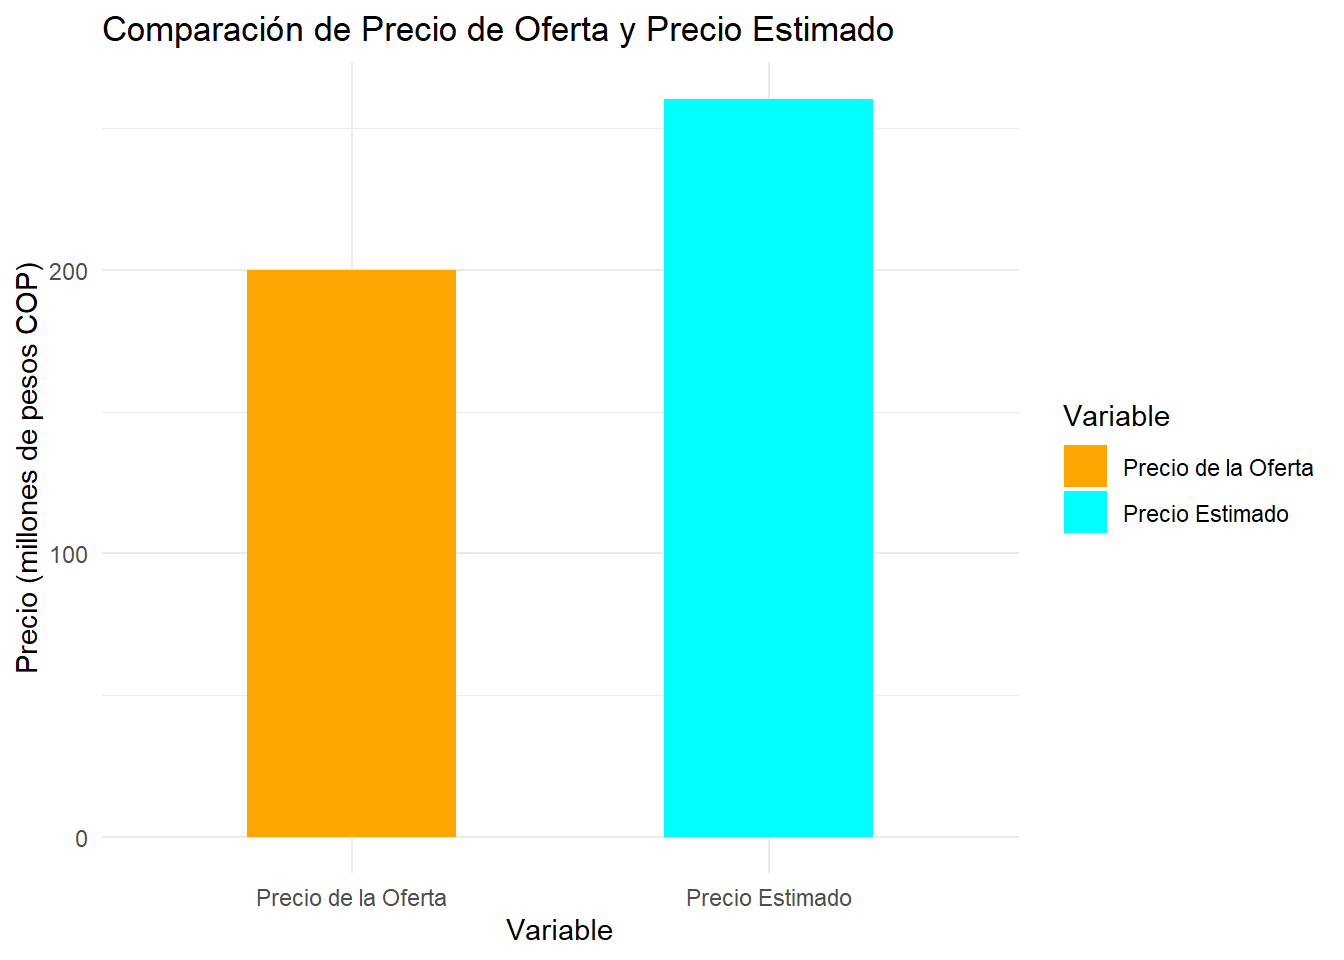
\includegraphics{Activdad_03_files/figure-latex/unnamed-chunk-40-1.pdf}

\section{\texorpdfstring{\textbf{7. Realice la validación de los
supuestos del modelo por medio de gráficos apropiados, interpretarlos y
sugerir posibles soluciones si se violan algunos de ellos. Utilice las
pruebas de hipótesis para la validación de supuestos y compare los
resultados con lo observado en los gráficos
asociados.}}{7. Realice la validación de los supuestos del modelo por medio de gráficos apropiados, interpretarlos y sugerir posibles soluciones si se violan algunos de ellos. Utilice las pruebas de hipótesis para la validación de supuestos y compare los resultados con lo observado en los gráficos asociados.}}\label{realice-la-validaciuxf3n-de-los-supuestos-del-modelo-por-medio-de-gruxe1ficos-apropiados-interpretarlos-y-sugerir-posibles-soluciones-si-se-violan-algunos-de-ellos.-utilice-las-pruebas-de-hipuxf3tesis-para-la-validaciuxf3n-de-supuestos-y-compare-los-resultados-con-lo-observado-en-los-gruxe1ficos-asociados.}

\begin{Shaded}
\begin{Highlighting}[]
\FunctionTok{par}\NormalTok{ (}\AttributeTok{mfrow=}\FunctionTok{c}\NormalTok{(}\DecValTok{2}\NormalTok{,}\DecValTok{2}\NormalTok{))}
\FunctionTok{plot}\NormalTok{(modelo\_regresion1)}
\end{Highlighting}
\end{Shaded}

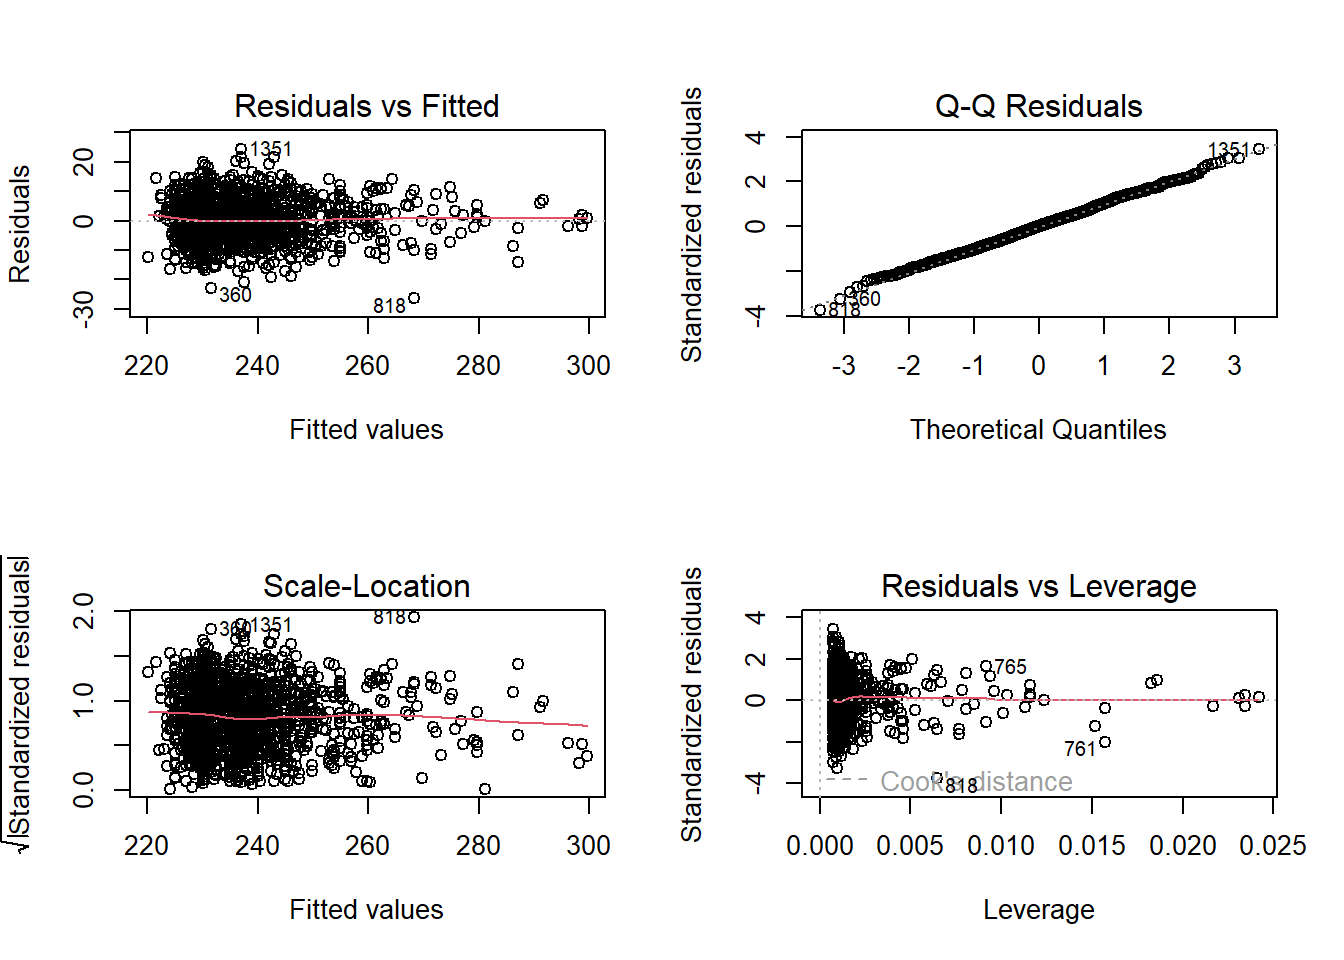
\includegraphics{Activdad_03_files/figure-latex/unnamed-chunk-41-1.pdf}

\begin{Shaded}
\begin{Highlighting}[]
\CommentTok{\# Gráfico de Residuales vs. Valores Ajustados}
\FunctionTok{plot}\NormalTok{(modelo\_regresion1, }\AttributeTok{which =} \DecValTok{1}\NormalTok{)}
\end{Highlighting}
\end{Shaded}

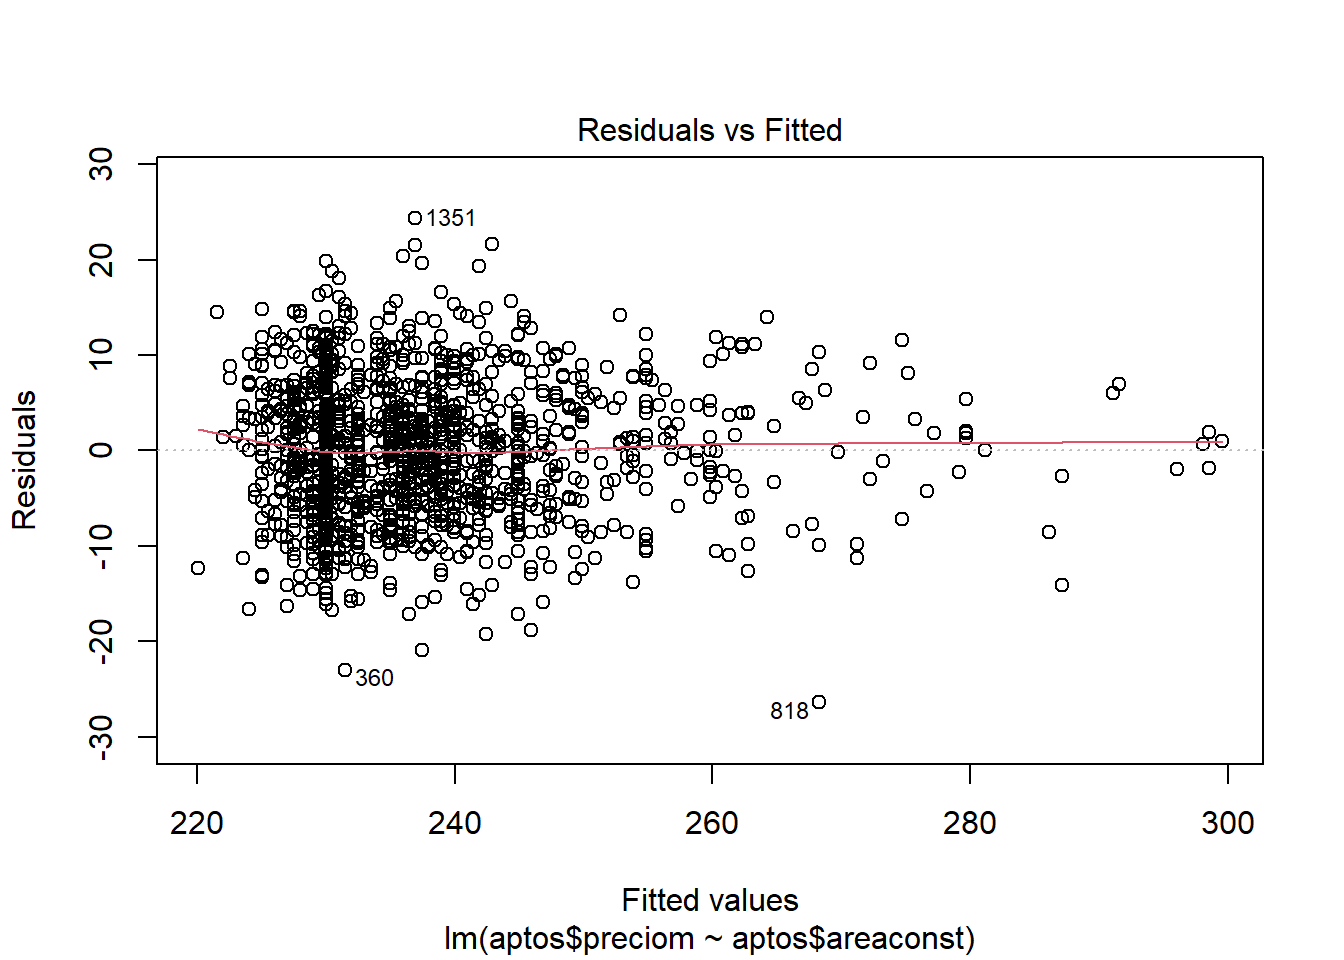
\includegraphics{Activdad_03_files/figure-latex/unnamed-chunk-42-1.pdf}

\begin{Shaded}
\begin{Highlighting}[]
\FunctionTok{durbinWatsonTest}\NormalTok{(modelo\_regresion1)}
\end{Highlighting}
\end{Shaded}

\begin{verbatim}
##  lag Autocorrelation D-W Statistic p-value
##    1      -0.0114037      2.022234   0.682
##  Alternative hypothesis: rho != 0
\end{verbatim}

\begin{Shaded}
\begin{Highlighting}[]
\CommentTok{\# Gráfico de Residuales vs. Orden}
\FunctionTok{plot}\NormalTok{(modelo\_regresion1, }\AttributeTok{which =} \DecValTok{2}\NormalTok{)}
\end{Highlighting}
\end{Shaded}

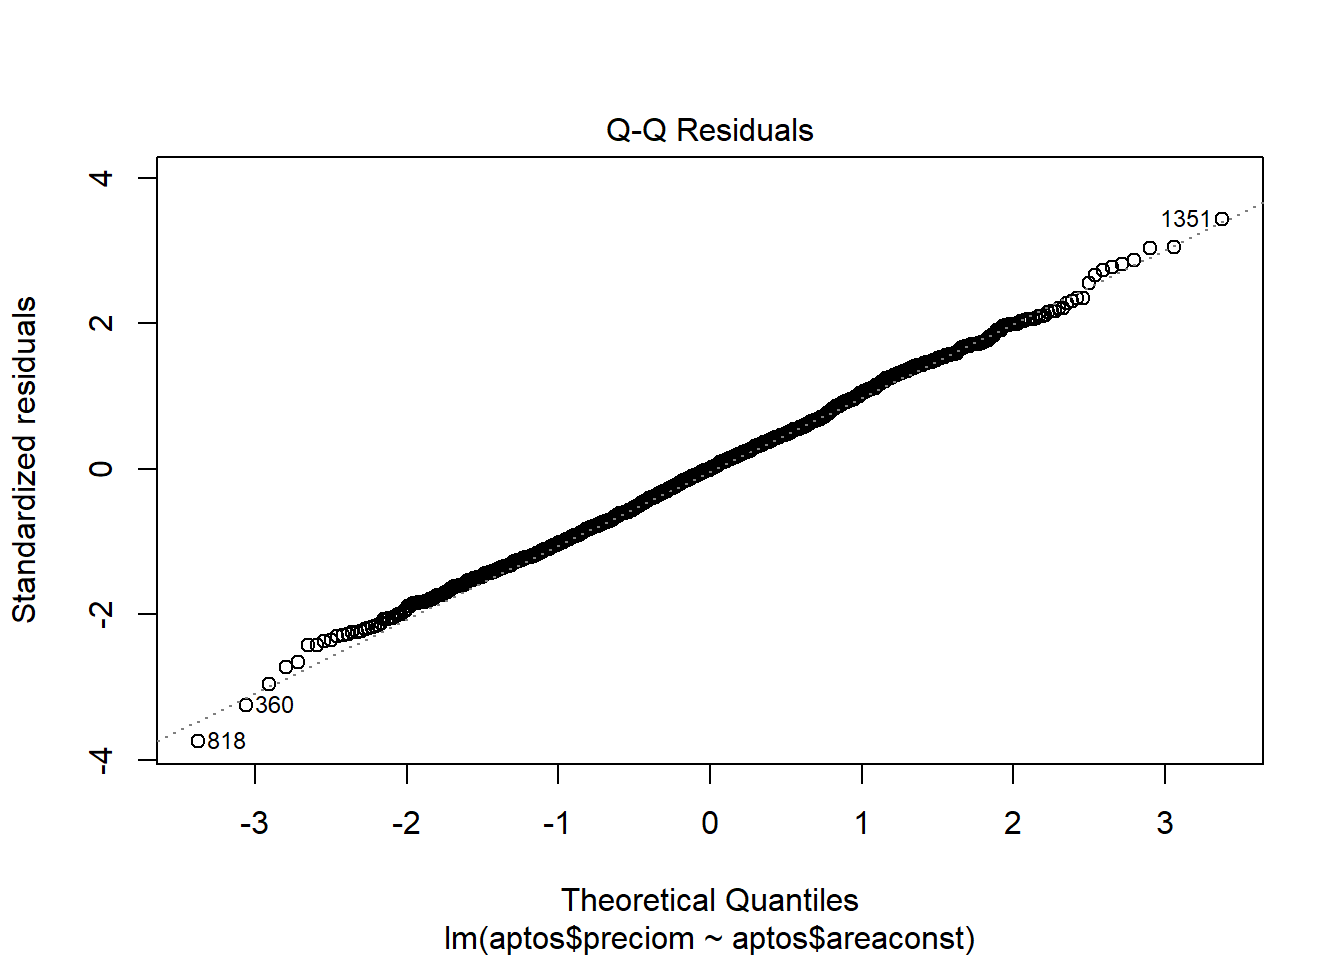
\includegraphics{Activdad_03_files/figure-latex/unnamed-chunk-44-1.pdf}

\begin{Shaded}
\begin{Highlighting}[]
\CommentTok{\# Prueba de Ljung{-}Box}
\FunctionTok{library}\NormalTok{(astsa)}
\FunctionTok{Box.test}\NormalTok{(}\FunctionTok{resid}\NormalTok{(modelo\_regresion1), }\AttributeTok{lag =} \DecValTok{20}\NormalTok{, }\AttributeTok{type =} \StringTok{"Ljung"}\NormalTok{)}
\end{Highlighting}
\end{Shaded}

\begin{verbatim}
## 
##  Box-Ljung test
## 
## data:  resid(modelo_regresion1)
## X-squared = 19.343, df = 20, p-value = 0.4997
\end{verbatim}

\begin{Shaded}
\begin{Highlighting}[]
\CommentTok{\# Gráfico Q{-}Q (Quantile{-}Quantile)}
\FunctionTok{qqnorm}\NormalTok{(}\FunctionTok{resid}\NormalTok{(modelo\_regresion1))}
\FunctionTok{qqline}\NormalTok{(}\FunctionTok{resid}\NormalTok{(modelo\_regresion1))}
\end{Highlighting}
\end{Shaded}

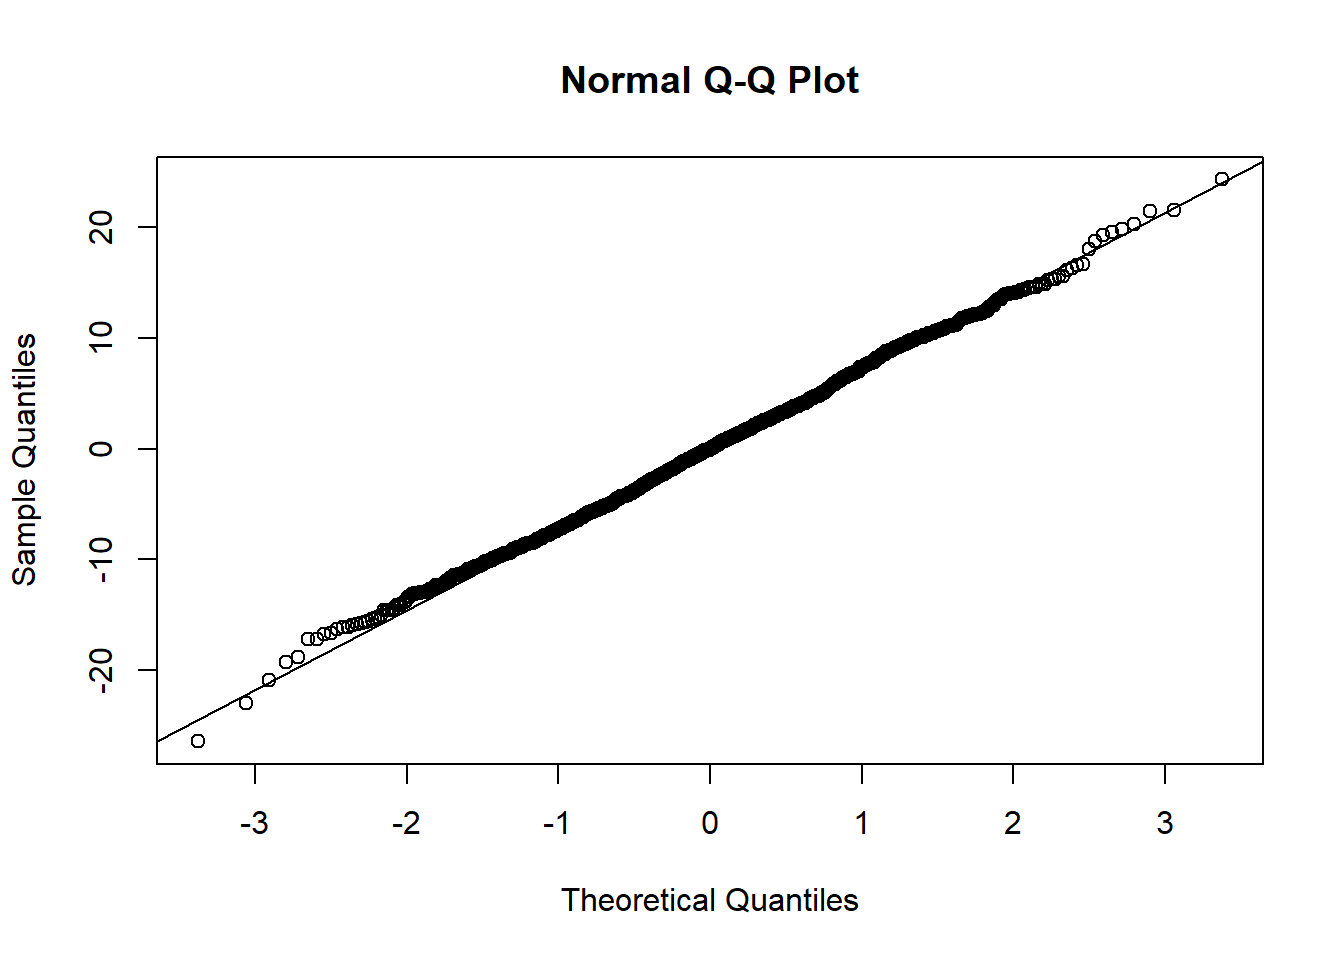
\includegraphics{Activdad_03_files/figure-latex/unnamed-chunk-46-1.pdf}

Para cada gráfica los hallazgos son los siguientes:

\subsection{\texorpdfstring{\textbf{7.1. Gráfico de
Linealidad}}{7.1. Gráfico de Linealidad}}\label{gruxe1fico-de-linealidad}

La gráfica de Residuals vs Fitted permite evaluar si los residuales
(errores) del modelo tienen una relación sistemática con los valores
ajustados (predichos).

En este caso, se observa que los residuales no presentan una dispersión
completamente aleatoria, lo que indica que no se cumple el supuesto de
linealidad. Además, se puede notar que la variabilidad de los errores no
es constante, lo que infringe el supuesto de homocedasticidad y de igual
forma, se aprecia una concentración mayor de errores hacia la izquierda,
sugiriendo una distribución asimétrica o algún patrón que podría afectar
la validez del modelo.

\subsection{\texorpdfstring{\textbf{7.2. Gráfico de
Normalidad}}{7.2. Gráfico de Normalidad}}\label{gruxe1fico-de-normalidad}

En el gráfico Q-Q, se observa que los puntos al inicio y al final se
desvían de la línea recta diagonal, lo que indica que los residuales del
modelo no siguen una distribución normal. Esto sugiere que las
inferencias estadísticas basadas en los supuestos de normalidad, como
las pruebas de hipótesis del modelo, pueden estar sesgadas. Sin embargo,
es importante destacar que, aunque los residuales no se ajusten
completamente a una distribución normal, en algunos casos, los modelos
aún pueden ofrecer predicciones útiles y fiables, dependiendo de la
magnitud del desajuste y de la aplicación práctica.

Lo anterior, es posible verificar por medio de la prueba de shapiro:

\begin{Shaded}
\begin{Highlighting}[]
\CommentTok{\# Prueba de Shapiro{-}Wilk}
\FunctionTok{shapiro.test}\NormalTok{(}\FunctionTok{resid}\NormalTok{(modelo\_regresion1))}
\end{Highlighting}
\end{Shaded}

\begin{verbatim}
## 
##  Shapiro-Wilk normality test
## 
## data:  resid(modelo_regresion1)
## W = 0.99884, p-value = 0.5279
\end{verbatim}

Teniendo en cuenta el resultado anterior, se puede evidenciar que los
residuales no siguen una distribución normal en el modelo

\subsection{\texorpdfstring{\textbf{7.3. Gráfico
Homocedasticidad}}{7.3. Gráfico Homocedasticidad}}\label{gruxe1fico-homocedasticidad}

Este tipo de gráfico nos permite examinar si la variabilidad de los
residuales es constante a lo largo de los valores ajustados. Se puede
observar que la dispersión de los residuos del modelo de apartamentos no
es uniforme alrededor de la línea de regresión, mostrando una mayor
dispersión a medida que aumentan los valores ajustados. Esto sugiere la
presencia de heterocedasticidad. Además, se aprecia que la varianza de
los residuos crece conforme incrementan los valores ajustados, lo que
implica una violación del supuesto de homocedasticidad.

\begin{Shaded}
\begin{Highlighting}[]
\NormalTok{lmtest}\SpecialCharTok{::}\FunctionTok{bptest}\NormalTok{(modelo\_regresion1)}
\end{Highlighting}
\end{Shaded}

\begin{verbatim}
## 
##  studentized Breusch-Pagan test
## 
## data:  modelo_regresion1
## BP = 0.62616, df = 1, p-value = 0.4288
\end{verbatim}

Al aplicar la prueba de Breusch-Pagan y observar un valor p
significativamente bajo, se concluye que hay evidencia suficiente para
rechazar la hipótesis nula de homocedasticidad. Esto confirma la
presencia de heterocedasticidad en los residuos del modelo, lo que
sugiere que la variabilidad de los errores no es constante a lo largo de
los valores ajustados.

\subsection{\texorpdfstring{\textbf{7.4. Gráfico de
Outliers}}{7.4. Gráfico de Outliers}}\label{gruxe1fico-de-outliers}

Con este gráfico podemos identificar observaciones atípicas (outlier).
Las observaciones con valores inusualmente extremos en las variables
predictoras pueden tener un alto impacto en las estimaciones de los
coeficientes del modelo. En el eje X vemos el leverage (medida de cuánto
se aleja el valor de una observación del valor promedio de las variables
predictoras) y en el eje Y se representan los residuales estandarizados.
Las observaciones que están lejos del resto de los puntos en el eje y
pueden ser consideradas atípicas. Con el gráfico generado, se observa
que sí hay valores extremos, aunque no es un supuesto formal, no se
esperaría que hayan datos atípicos que generen sesgos en los estimadores
de los coeficientes.

\subsection{\texorpdfstring{\textbf{7.5. No
autocorrelación}}{7.5. No autocorrelación}}\label{no-autocorrelaciuxf3n}

\begin{Shaded}
\begin{Highlighting}[]
\NormalTok{lmtest}\SpecialCharTok{::}\FunctionTok{dwtest}\NormalTok{(modelo\_regresion1)}
\end{Highlighting}
\end{Shaded}

\begin{verbatim}
## 
##  Durbin-Watson test
## 
## data:  modelo_regresion1
## DW = 2.0222, p-value = 0.6557
## alternative hypothesis: true autocorrelation is greater than 0
\end{verbatim}

Los errores que corresponden a diferentes individuos o factores deben
ser independientes entre sí, lo que implica que la covarianza entre
ellos (Cov{[}εi, εj{]}) debe ser igual a 0. El \textbf{test de
Durbin-Watson} de primer orden, cuyo rango va de 0 a 4, ayuda a detectar
la autocorrelación en los residuos.

Un valor cercano a 2 indica la ausencia de autocorrelación positiva o
negativa. Si el valor es significativamente menor que 2, sugiere
autocorrelación positiva. Según el criterio, valores entre 1.54 y 2.45
indican la no existencia de autocorrelación.

El valor de \textbf{2.02} obtenido en la prueba para este modelo indica
que no hay autocorrelación positiva en los residuos, confirmando que los
errores no están correlacionados positivamente entre sí.

\section{\texorpdfstring{\textbf{8. De ser necesario realice una
transformación apropiada para mejorar el ajuste y supuestos del
modelo.}}{8. De ser necesario realice una transformación apropiada para mejorar el ajuste y supuestos del modelo.}}\label{de-ser-necesario-realice-una-transformaciuxf3n-apropiada-para-mejorar-el-ajuste-y-supuestos-del-modelo.}

\subsection{\texorpdfstring{\textbf{8.1. Transformación
Lin-Log}}{8.1. Transformación Lin-Log}}\label{transformaciuxf3n-lin-log}

\begin{Shaded}
\begin{Highlighting}[]
\NormalTok{modelo\_LinLog }\OtherTok{=} \FunctionTok{lm}\NormalTok{(preciom }\SpecialCharTok{\textasciitilde{}} \FunctionTok{log}\NormalTok{(areaconst), }\AttributeTok{data=}\NormalTok{aptos)      }
\FunctionTok{summary}\NormalTok{(modelo\_LinLog)}
\end{Highlighting}
\end{Shaded}

\begin{verbatim}
## 
## Call:
## lm(formula = preciom ~ log(areaconst), data = aptos)
## 
## Residuals:
##      Min       1Q   Median       3Q      Max 
## -23.0149  -5.3820  -0.1439   4.9163  22.9510 
## 
## Coefficients:
##                Estimate Std. Error t value Pr(>|t|)    
## (Intercept)     56.0556     3.4259   16.36   <2e-16 ***
## log(areaconst)  42.3485     0.7978   53.08   <2e-16 ***
## ---
## Signif. codes:  0 '***' 0.001 '**' 0.01 '*' 0.05 '.' 0.1 ' ' 1
## 
## Residual standard error: 7.449 on 1359 degrees of freedom
## Multiple R-squared:  0.6746, Adjusted R-squared:  0.6744 
## F-statistic:  2818 on 1 and 1359 DF,  p-value: < 2.2e-16
\end{verbatim}

\begin{Shaded}
\begin{Highlighting}[]
\FunctionTok{par}\NormalTok{ (}\AttributeTok{mfrow=}\FunctionTok{c}\NormalTok{(}\DecValTok{2}\NormalTok{,}\DecValTok{2}\NormalTok{))}
\FunctionTok{plot}\NormalTok{(modelo\_LinLog)}
\end{Highlighting}
\end{Shaded}

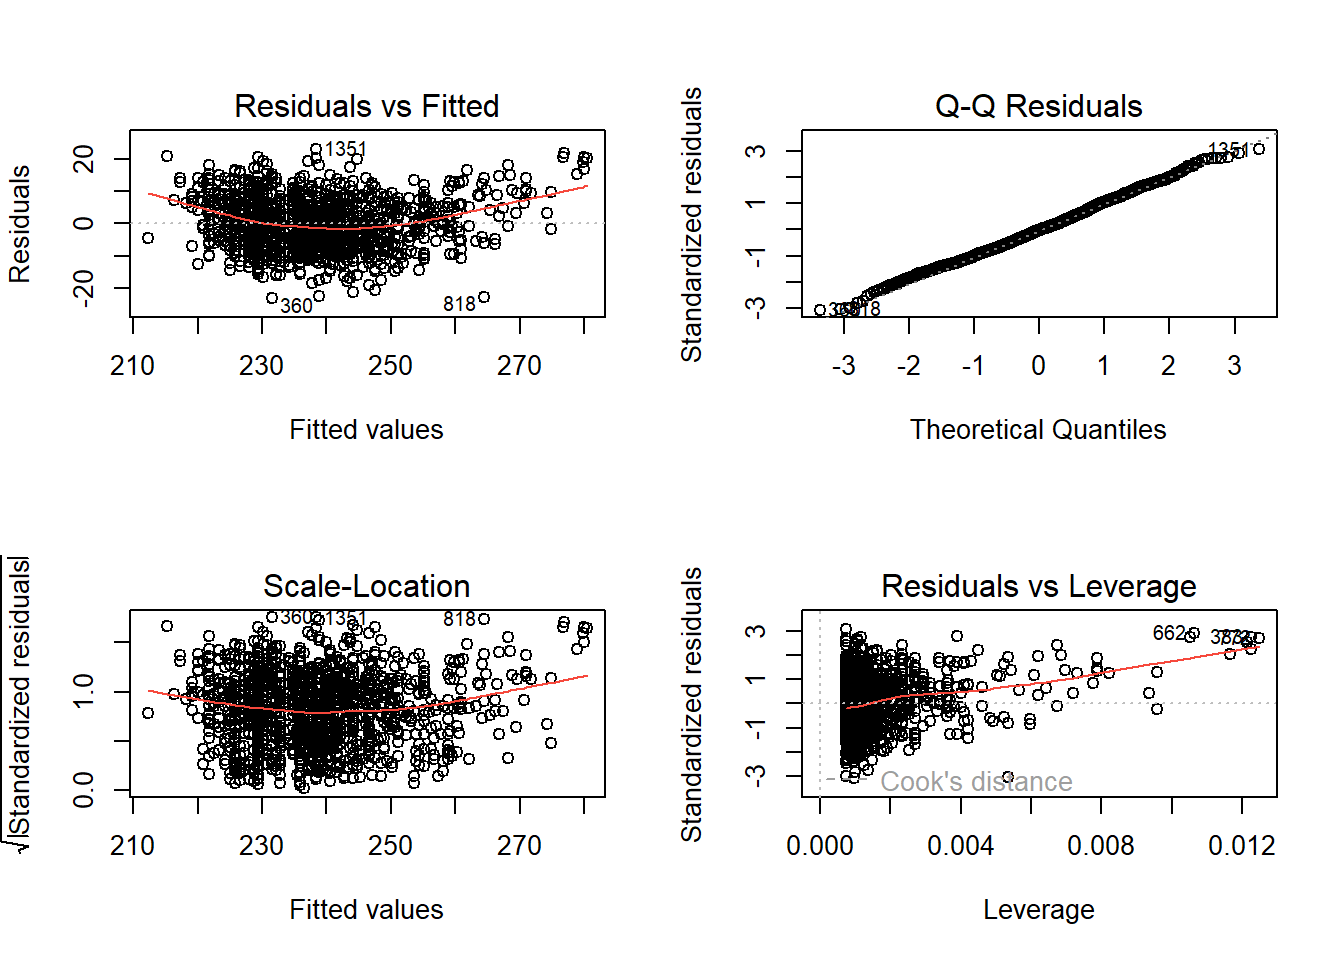
\includegraphics{Activdad_03_files/figure-latex/unnamed-chunk-50-1.pdf}

Al haber realizado la transformación logarítmica de la
\textbf{\emph{variable X}}, los resultados muestran que, tras aplicar la
transformación Lin-Log, el valor del R² disminuye a \textbf{\emph{0.68}}
aproximadamente, en comparación con el modelo inicial. Sin embargo, a
pesar de la reducción en R², el modelo sigue siendo significativo, como
lo indica el estadístico p-value, lo cual sugiere que la relación entre
las variables sigue siendo estadísticamente relevante.

\subsection{\texorpdfstring{\textbf{8.1. Transformación
Lin-Log}}{8.1. Transformación Lin-Log}}\label{transformaciuxf3n-lin-log-1}

\begin{Shaded}
\begin{Highlighting}[]
\NormalTok{modelo\_LogLin }\OtherTok{=} \FunctionTok{lm}\NormalTok{(}\FunctionTok{log}\NormalTok{(preciom) }\SpecialCharTok{\textasciitilde{}}\NormalTok{ areaconst, }\AttributeTok{data=}\NormalTok{aptos)      }
\FunctionTok{summary}\NormalTok{(modelo\_LogLin)}
\end{Highlighting}
\end{Shaded}

\begin{verbatim}
## 
## Call:
## lm(formula = log(preciom) ~ areaconst, data = aptos)
## 
## Residuals:
##       Min        1Q    Median        3Q       Max 
## -0.104718 -0.020997  0.000605  0.019349  0.099107 
## 
## Coefficients:
##              Estimate Std. Error t value Pr(>|t|)    
## (Intercept) 5.318e+00  2.891e-03  1839.7   <2e-16 ***
## areaconst   2.008e-03  3.684e-05    54.5   <2e-16 ***
## ---
## Signif. codes:  0 '***' 0.001 '**' 0.01 '*' 0.05 '.' 0.1 ' ' 1
## 
## Residual standard error: 0.02999 on 1359 degrees of freedom
## Multiple R-squared:  0.6861, Adjusted R-squared:  0.6858 
## F-statistic:  2970 on 1 and 1359 DF,  p-value: < 2.2e-16
\end{verbatim}

\begin{Shaded}
\begin{Highlighting}[]
\FunctionTok{par}\NormalTok{ (}\AttributeTok{mfrow=}\FunctionTok{c}\NormalTok{(}\DecValTok{2}\NormalTok{,}\DecValTok{2}\NormalTok{))}
\FunctionTok{plot}\NormalTok{(modelo\_LogLin)}
\end{Highlighting}
\end{Shaded}

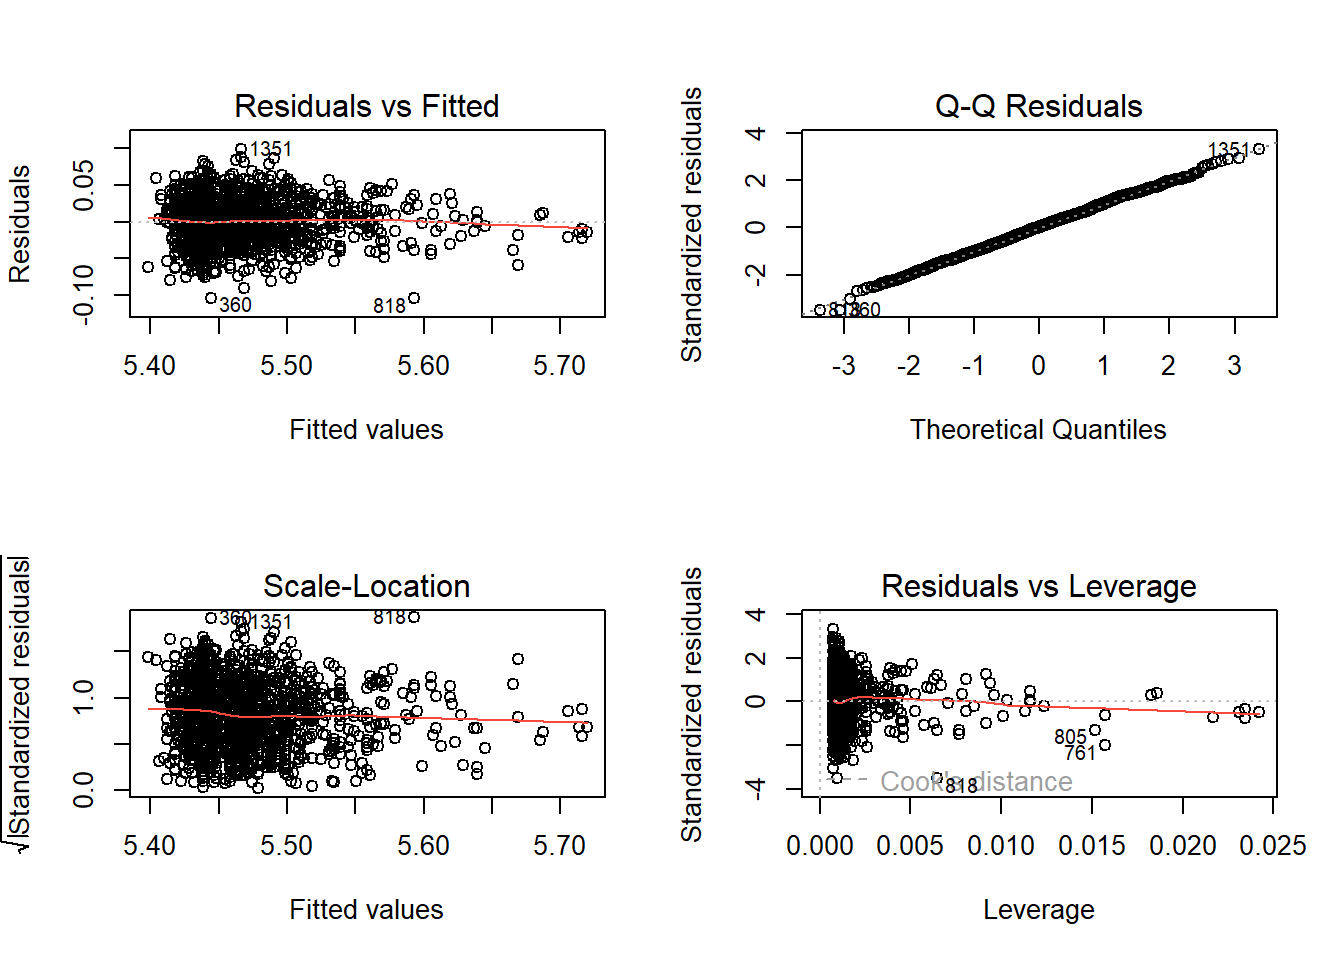
\includegraphics{Activdad_03_files/figure-latex/unnamed-chunk-51-1.pdf}

Al haber realizado la transformación logarítmica de la
\textbf{\emph{variable Y}}, los resultados muestran que,la
transformación Log-Lin produce un valor de R² de apróximadamente
\textbf{\emph{0.69}} ligeramente inferior al del modelo original. Aunque
también se reduce el R², el modelo sigue siendo significativo, como lo
indica el estadístico valor de p (p-value), confirmando así la relación
que existe entre las variables continúa siendo estadísticamente
relevante.

\subsection{\texorpdfstring{\textbf{8.3. Transformación
Log-Log}}{8.3. Transformación Log-Log}}\label{transformaciuxf3n-log-log}

\begin{Shaded}
\begin{Highlighting}[]
\NormalTok{modelo\_LogLog }\OtherTok{=} \FunctionTok{lm}\NormalTok{(}\FunctionTok{log}\NormalTok{(preciom) }\SpecialCharTok{\textasciitilde{}} \FunctionTok{log}\NormalTok{(areaconst), }\AttributeTok{data=}\NormalTok{aptos) }
\FunctionTok{summary}\NormalTok{(modelo\_LogLog)}
\end{Highlighting}
\end{Shaded}

\begin{verbatim}
## 
## Call:
## lm(formula = log(preciom) ~ log(areaconst), data = aptos)
## 
## Residuals:
##       Min        1Q    Median        3Q       Max 
## -0.104409 -0.022224  0.000044  0.020791  0.093492 
## 
## Coefficients:
##                Estimate Std. Error t value Pr(>|t|)    
## (Intercept)     4.72964    0.01421  332.74   <2e-16 ***
## log(areaconst)  0.17250    0.00331   52.11   <2e-16 ***
## ---
## Signif. codes:  0 '***' 0.001 '**' 0.01 '*' 0.05 '.' 0.1 ' ' 1
## 
## Residual standard error: 0.03091 on 1359 degrees of freedom
## Multiple R-squared:  0.6665, Adjusted R-squared:  0.6662 
## F-statistic:  2716 on 1 and 1359 DF,  p-value: < 2.2e-16
\end{verbatim}

\begin{Shaded}
\begin{Highlighting}[]
\FunctionTok{par}\NormalTok{ (}\AttributeTok{mfrow=}\FunctionTok{c}\NormalTok{(}\DecValTok{2}\NormalTok{,}\DecValTok{2}\NormalTok{))}
\FunctionTok{plot}\NormalTok{(modelo\_LogLog)}
\end{Highlighting}
\end{Shaded}

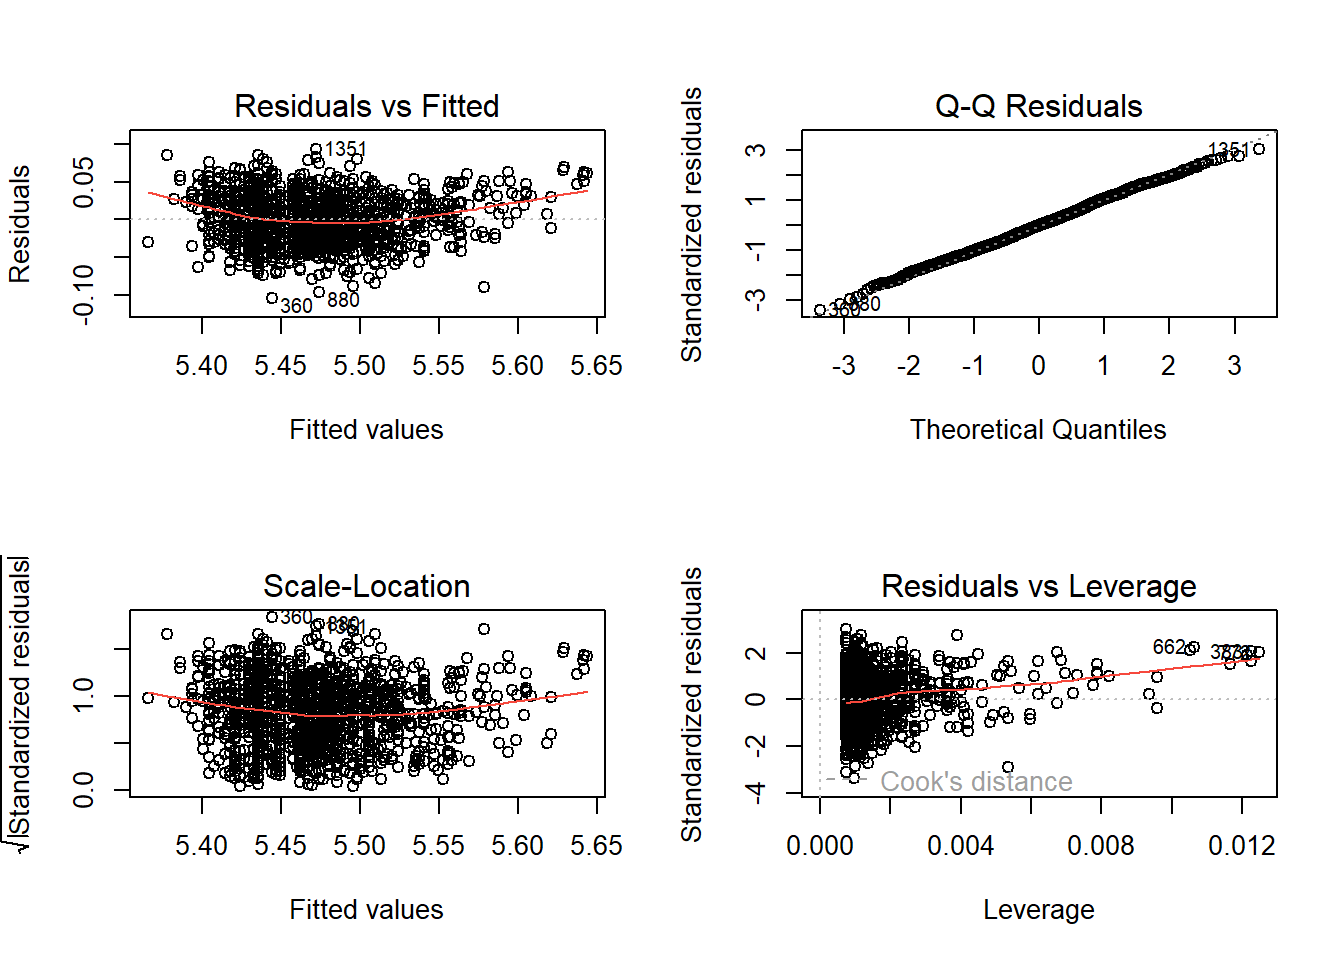
\includegraphics{Activdad_03_files/figure-latex/unnamed-chunk-52-1.pdf}

Al haber realizado la transformación logarítmica de la
\textbf{\emph{variable X}} y la \textbf{\emph{variable Y}}, los
resultados muestran que con la transformación Log-Log, el valor de R²
disminuye a \textbf{\emph{0.67}} apróximadamente, siendo inferior al del
modelo original y a los modelos Lin-Log y Log-Lin. No obstante, el
estadístico p-value sigue siendo significativo, lo que indica que la
relación entre las variables, aunque menos explicativa en comparación
con los otros modelos, sigue siendo estadísticamente significativa.

\subsection{\texorpdfstring{\textbf{8.4. Transformación
Box-Cox}}{8.4. Transformación Box-Cox}}\label{transformaciuxf3n-box-cox}

\begin{Shaded}
\begin{Highlighting}[]
\CommentTok{\# Instalar paquetes si no están instalados}
\ControlFlowTok{if}\NormalTok{(}\SpecialCharTok{!}\FunctionTok{require}\NormalTok{(MASS)) }\FunctionTok{install.packages}\NormalTok{(}\StringTok{"MASS"}\NormalTok{)}
\end{Highlighting}
\end{Shaded}

\begin{verbatim}
## Loading required package: MASS
\end{verbatim}

\begin{verbatim}
## 
## Attaching package: 'MASS'
\end{verbatim}

\begin{verbatim}
## The following object is masked from 'package:dplyr':
## 
##     select
\end{verbatim}

\begin{Shaded}
\begin{Highlighting}[]
\ControlFlowTok{if}\NormalTok{(}\SpecialCharTok{!}\FunctionTok{require}\NormalTok{(car)) }\FunctionTok{install.packages}\NormalTok{(}\StringTok{"car"}\NormalTok{)}
\ControlFlowTok{if}\NormalTok{(}\SpecialCharTok{!}\FunctionTok{require}\NormalTok{(lmtest)) }\FunctionTok{install.packages}\NormalTok{(}\StringTok{"lmtest"}\NormalTok{)}

\CommentTok{\# Cargar la librería MASS para la transformación de Box{-}Cox}
\FunctionTok{library}\NormalTok{(MASS)}
\NormalTok{modelo\_regresion1 }\OtherTok{=} \FunctionTok{lm}\NormalTok{(preciom }\SpecialCharTok{\textasciitilde{}}\NormalTok{ areaconst, }\AttributeTok{data=}\NormalTok{aptos)}
\FunctionTok{summary}\NormalTok{(modelo\_regresion1)}
\end{Highlighting}
\end{Shaded}

\begin{verbatim}
## 
## Call:
## lm(formula = preciom ~ areaconst, data = aptos)
## 
## Residuals:
##      Min       1Q   Median       3Q      Max 
## -26.4137  -5.0770  -0.0061   4.6197  24.3348 
## 
## Coefficients:
##              Estimate Std. Error t value Pr(>|t|)    
## (Intercept) 2.002e+02  6.829e-01  293.11   <2e-16 ***
## areaconst   4.969e-01  8.704e-03   57.09   <2e-16 ***
## ---
## Signif. codes:  0 '***' 0.001 '**' 0.01 '*' 0.05 '.' 0.1 ' ' 1
## 
## Residual standard error: 7.084 on 1359 degrees of freedom
## Multiple R-squared:  0.7057, Adjusted R-squared:  0.7055 
## F-statistic:  3259 on 1 and 1359 DF,  p-value: < 2.2e-16
\end{verbatim}

\begin{Shaded}
\begin{Highlighting}[]
\FunctionTok{par}\NormalTok{(}\AttributeTok{mfrow =} \FunctionTok{c}\NormalTok{(}\DecValTok{1}\NormalTok{,}\DecValTok{2}\NormalTok{))}
\FunctionTok{boxcox}\NormalTok{( }\FunctionTok{lm}\NormalTok{( aptos}\SpecialCharTok{$}\NormalTok{preciom }\SpecialCharTok{\textasciitilde{}}\NormalTok{ aptos}\SpecialCharTok{$}\NormalTok{areaconst, }\AttributeTok{data=}\NormalTok{aptos ), }\AttributeTok{lambda =} \SpecialCharTok{{-}}\DecValTok{3}\SpecialCharTok{:}\DecValTok{3}\NormalTok{)}
\NormalTok{graficoBoxcox }\OtherTok{\textless{}{-}} \FunctionTok{boxcox}\NormalTok{( }\FunctionTok{lm}\NormalTok{( aptos}\SpecialCharTok{$}\NormalTok{preciom }\SpecialCharTok{\textasciitilde{}}\NormalTok{ aptos}\SpecialCharTok{$}\NormalTok{areaconst, }\AttributeTok{data=}\NormalTok{aptos ), }\AttributeTok{lambda =} \SpecialCharTok{{-}}\DecValTok{1}\SpecialCharTok{:}\DecValTok{1}\NormalTok{)}
\end{Highlighting}
\end{Shaded}

\includegraphics{Activdad_03_files/figure-latex/unnamed-chunk-53-1.pdf}

\begin{Shaded}
\begin{Highlighting}[]
\NormalTok{(lambda }\OtherTok{\textless{}{-}}\NormalTok{ graficoBoxcox}\SpecialCharTok{$}\NormalTok{x[}\FunctionTok{which.max}\NormalTok{( graficoBoxcox}\SpecialCharTok{$}\NormalTok{y )])}
\end{Highlighting}
\end{Shaded}

\begin{verbatim}
## [1] 1
\end{verbatim}

\begin{Shaded}
\begin{Highlighting}[]
\NormalTok{Y\_Ajustado }\OtherTok{\textless{}{-}}\NormalTok{ ((aptos}\SpecialCharTok{$}\NormalTok{preciom }\SpecialCharTok{\^{}}\NormalTok{ lambda) }\SpecialCharTok{{-}}\DecValTok{1}\NormalTok{)}\SpecialCharTok{/}\NormalTok{ lambda}
\NormalTok{modeloBoxCox }\OtherTok{\textless{}{-}} \FunctionTok{lm}\NormalTok{(Y\_Ajustado}\SpecialCharTok{\textasciitilde{}}\NormalTok{areaconst, }\AttributeTok{data=}\NormalTok{aptos)}

\FunctionTok{summary}\NormalTok{(modeloBoxCox)}
\end{Highlighting}
\end{Shaded}

\begin{verbatim}
## 
## Call:
## lm(formula = Y_Ajustado ~ areaconst, data = aptos)
## 
## Residuals:
##      Min       1Q   Median       3Q      Max 
## -26.4137  -5.0770  -0.0061   4.6197  24.3348 
## 
## Coefficients:
##              Estimate Std. Error t value Pr(>|t|)    
## (Intercept) 1.992e+02  6.829e-01  291.64   <2e-16 ***
## areaconst   4.969e-01  8.704e-03   57.09   <2e-16 ***
## ---
## Signif. codes:  0 '***' 0.001 '**' 0.01 '*' 0.05 '.' 0.1 ' ' 1
## 
## Residual standard error: 7.084 on 1359 degrees of freedom
## Multiple R-squared:  0.7057, Adjusted R-squared:  0.7055 
## F-statistic:  3259 on 1 and 1359 DF,  p-value: < 2.2e-16
\end{verbatim}

\begin{Shaded}
\begin{Highlighting}[]
\FunctionTok{par}\NormalTok{ (}\AttributeTok{mfrow=}\FunctionTok{c}\NormalTok{(}\DecValTok{2}\NormalTok{,}\DecValTok{2}\NormalTok{))}
\FunctionTok{plot}\NormalTok{(modeloBoxCox)}
\end{Highlighting}
\end{Shaded}

\includegraphics{Activdad_03_files/figure-latex/unnamed-chunk-54-1.pdf}

Sabemos que la transformación sobre la variable Y se utiliza comúnmente
para abordar problemas relacionados con la validación de supuestos y
para mejorar el ajuste del modelo. En este caso, se obtiene un lambda
con valor de uno y en ambas gráficas, el intervalo de confianza se
incluye el valor de 1. Este resultado, \textbf{\emph{λ = 1}}, sugiere
que la variable dependiente no necesita estar en escala logarítmica, por
lo que no es necesario realizar dicha transformación.

\subsubsection{Tabla comparativa de
modelos}\label{tabla-comparativa-de-modelos}

\begin{Shaded}
\begin{Highlighting}[]
\FunctionTok{library}\NormalTok{ (stargazer)}
\end{Highlighting}
\end{Shaded}

\begin{verbatim}
## 
## Please cite as:
\end{verbatim}

\begin{verbatim}
##  Hlavac, Marek (2022). stargazer: Well-Formatted Regression and Summary Statistics Tables.
\end{verbatim}

\begin{verbatim}
##  R package version 5.2.3. https://CRAN.R-project.org/package=stargazer
\end{verbatim}

\begin{Shaded}
\begin{Highlighting}[]
\FunctionTok{stargazer}\NormalTok{(modelo\_regresion1, modelo\_LinLog, modelo\_LogLin, modelo\_LogLog, }\AttributeTok{type =} \StringTok{"text"}\NormalTok{, }\AttributeTok{df=}\ConstantTok{FALSE}\NormalTok{, }\AttributeTok{title =} \StringTok{"Tabla comparativa de modelos"}\NormalTok{)}
\end{Highlighting}
\end{Shaded}

\begin{verbatim}
## 
## Tabla comparativa de modelos
## =======================================================================
##                                     Dependent variable:                
##                     ---------------------------------------------------
##                              preciom                log(preciom)       
##                         (1)          (2)          (3)          (4)     
## -----------------------------------------------------------------------
## areaconst             0.497***                  0.002***               
##                       (0.009)                  (0.00004)               
##                                                                        
## log(areaconst)                    42.348***                  0.172***  
##                                    (0.798)                   (0.003)   
##                                                                        
## Constant             200.173***   56.056***     5.318***     4.730***  
##                       (0.683)      (3.426)      (0.003)      (0.014)   
##                                                                        
## -----------------------------------------------------------------------
## Observations           1,361        1,361        1,361        1,361    
## R2                     0.706        0.675        0.686        0.666    
## Adjusted R2            0.705        0.674        0.686        0.666    
## Residual Std. Error    7.084        7.449        0.030        0.031    
## F Statistic         3,258.889*** 2,817.550*** 2,969.799*** 2,715.600***
## =======================================================================
## Note:                                       *p<0.1; **p<0.05; ***p<0.01
\end{verbatim}

Luego de haber realizado las transformaciones correspondientes tanto a
la variable independiente \textbf{\emph{(areaconst)}} como en la
dependiente \textbf{\emph{(Preciom)}}, para el tipo de vivienda
apartamentos y de haber comparado los modelos, es posible determinar que
el \textbf{modelo 1} de regresión simple proporciona los mejores
resultados para la variable dependiente, dado que presenta un R² de
70.6\%, siendo superior a los modelos con transformaciones e indicando
de igual forma que el \textbf{área construida} tiene una mayor
influencia en el precio.

Por otro lado, el modelo 1 de regresión lineal explica de una forma más
precisa y con un mayor ajuste en cuanto al precio en función del área
construída, específicamente en un 3.033\% más.

\section{\texorpdfstring{\textbf{9 y 10. Estime varios modelos y compare
los resultados obtenidos. En el mejor de los modelos, ¿Se cumplen los
supuestos sobre los
errores?}}{9 y 10. Estime varios modelos y compare los resultados obtenidos. En el mejor de los modelos, ¿Se cumplen los supuestos sobre los errores?}}\label{y-10.-estime-varios-modelos-y-compare-los-resultados-obtenidos.-en-el-mejor-de-los-modelos-se-cumplen-los-supuestos-sobre-los-errores}

\subsection{\texorpdfstring{\textbf{10.1. Coeficientes de
determinación:}}{10.1. Coeficientes de determinación:}}\label{coeficientes-de-determinaciuxf3n}

\begin{Shaded}
\begin{Highlighting}[]
\NormalTok{RSquared\_LinLog }\OtherTok{\textless{}{-}} \FunctionTok{summary}\NormalTok{(modelo\_LinLog)}\SpecialCharTok{$}\NormalTok{r.squared}
\NormalTok{RSquared\_LogLin }\OtherTok{\textless{}{-}} \FunctionTok{summary}\NormalTok{(modelo\_LogLin)}\SpecialCharTok{$}\NormalTok{r.squared}
\NormalTok{RSquared\_LogLog }\OtherTok{\textless{}{-}} \FunctionTok{summary}\NormalTok{(modelo\_LogLog)}\SpecialCharTok{$}\NormalTok{r.squared}
\NormalTok{RSquared\_BoxCox }\OtherTok{\textless{}{-}} \FunctionTok{summary}\NormalTok{(modeloBoxCox)}\SpecialCharTok{$}\NormalTok{r.squared}
\FunctionTok{print}\NormalTok{(}\FunctionTok{paste}\NormalTok{(}\StringTok{"Coeficiente de determinación Modelo lin{-}Log: "}\NormalTok{, RSquared\_LinLog))}
\end{Highlighting}
\end{Shaded}

\begin{verbatim}
## [1] "Coeficiente de determinación Modelo lin-Log:  0.674611816757162"
\end{verbatim}

\begin{Shaded}
\begin{Highlighting}[]
\FunctionTok{print}\NormalTok{(}\FunctionTok{paste}\NormalTok{(}\StringTok{"Coeficiente de determinación Modelo Log{-}Lin: "}\NormalTok{, RSquared\_LogLin))}
\end{Highlighting}
\end{Shaded}

\begin{verbatim}
## [1] "Coeficiente de determinación Modelo Log-Lin:  0.686056129804771"
\end{verbatim}

\begin{Shaded}
\begin{Highlighting}[]
\FunctionTok{print}\NormalTok{(}\FunctionTok{paste}\NormalTok{(}\StringTok{"Coeficiente de determinación Modelo Log{-}Log: "}\NormalTok{,RSquared\_LogLog))}
\end{Highlighting}
\end{Shaded}

\begin{verbatim}
## [1] "Coeficiente de determinación Modelo Log-Log:  0.666470329007742"
\end{verbatim}

\begin{Shaded}
\begin{Highlighting}[]
\FunctionTok{print}\NormalTok{(}\FunctionTok{paste}\NormalTok{(}\StringTok{"Coeficiente de determinación Modelo Box Cox: "}\NormalTok{, RSquared\_BoxCox))}
\end{Highlighting}
\end{Shaded}

\begin{verbatim}
## [1] "Coeficiente de determinación Modelo Box Cox:  0.705709661665464"
\end{verbatim}

\subsection{\texorpdfstring{\textbf{10.2.
Supuestos}}{10.2. Supuestos}}\label{supuestos}

\subsection{\texorpdfstring{\textbf{Normalidad:}}{Normalidad:}}\label{normalidad}

\begin{Shaded}
\begin{Highlighting}[]
\FunctionTok{par}\NormalTok{ (}\AttributeTok{mfrow=}\FunctionTok{c}\NormalTok{(}\DecValTok{2}\NormalTok{,}\DecValTok{3}\NormalTok{))}
\FunctionTok{qqnorm}\NormalTok{(modelo\_regresion1}\SpecialCharTok{$}\NormalTok{residuals, }\AttributeTok{main =} \StringTok{"Q{-}Q Modelo Original"}\NormalTok{, }\AttributeTok{col =} \StringTok{"blue"}\NormalTok{)}
\FunctionTok{qqline}\NormalTok{(modelo\_regresion1}\SpecialCharTok{$}\NormalTok{residuals)}

\FunctionTok{qqnorm}\NormalTok{(modelo\_LinLog}\SpecialCharTok{$}\NormalTok{residuals, }\AttributeTok{main =} \StringTok{"Q{-}Q Modelo Lin{-}Log"}\NormalTok{, }\AttributeTok{col =} \StringTok{"red"}\NormalTok{)}
\FunctionTok{qqline}\NormalTok{(modelo\_LinLog}\SpecialCharTok{$}\NormalTok{residuals)}

\FunctionTok{qqnorm}\NormalTok{(modelo\_LogLin}\SpecialCharTok{$}\NormalTok{residuals, }\AttributeTok{main =} \StringTok{"Q{-}Q Modelo Log{-}Lin"}\NormalTok{, }\AttributeTok{col =} \StringTok{"green"}\NormalTok{)}
\FunctionTok{qqline}\NormalTok{(modelo\_LogLin}\SpecialCharTok{$}\NormalTok{residuals)}

\FunctionTok{qqnorm}\NormalTok{(modelo\_LogLog}\SpecialCharTok{$}\NormalTok{residuals, }\AttributeTok{main =} \StringTok{"Q{-}Q Modelo Log{-}Log"}\NormalTok{, }\AttributeTok{col =} \StringTok{"gray"}\NormalTok{)}
\FunctionTok{qqline}\NormalTok{(modelo\_LogLog}\SpecialCharTok{$}\NormalTok{residuals)}

\FunctionTok{qqnorm}\NormalTok{(modeloBoxCox}\SpecialCharTok{$}\NormalTok{residuals, }\AttributeTok{main =} \StringTok{"Q{-}Q Modelo Box Cox"}\NormalTok{, }\AttributeTok{col =} \StringTok{"orange"}\NormalTok{)}
\FunctionTok{qqline}\NormalTok{(modeloBoxCox}\SpecialCharTok{$}\NormalTok{residuals)}
\end{Highlighting}
\end{Shaded}

\includegraphics{Activdad_03_files/figure-latex/unnamed-chunk-57-1.pdf}

Al observar los gráficos Q-Q de los cinco modelos (Original, Lin-Log,
Log-Lin, Log-Log, y Box-Cox), podemos notar lo siguiente:

\begin{itemize}
\item
  \textbf{Modelo Original:} Aunque la mayoría de los puntos siguen de
  cerca la línea diagonal, los extremos se desvían, lo que indica que
  los residuales no siguen una distribución normal. Esto sugiere la
  presencia de datos atípicos o colas más pesadas de lo esperado en los
  extremos de la distribución.
\item
  \textbf{Modelo Lin-Log y Log-Lin:} Estas transformaciones no lograron
  mejorar significativamente la normalidad. Aunque hay una mejor
  alineación de los puntos en el centro, los extremos aún presentan una
  notable desviación respecto a la línea de referencia, lo que implica
  que los residuales siguen sin ajustarse bien a una distribución
  normal.
\item
  \textbf{Modelo Log-Log:} Similar a los modelos anteriores, la
  transformación Log-Log tampoco muestra una mejora significativa en la
  distribución de los residuales. Los puntos en los extremos continúan
  desviándose, sugiriendo que los problemas de normalidad persisten.
\item
  \textbf{Modelo Box-Cox:} Aunque esta transformación está diseñada para
  mejorar la normalidad y homocedasticidad de los errores, el gráfico
  muestra que aún persisten desviaciones en los extremos. Sin embargo,
  este modelo presenta el mejor ajuste en la parte central en
  comparación con los otros, pero no es suficiente para garantizar
  normalidad.
\end{itemize}

\textbf{Conclusión:} Ninguno de los modelos transformados, incluyendo el
Box-Cox, ha sido capaz de corregir completamente la falta de normalidad
en los residuales. Esto podría indicar que los problemas en la
distribución de los errores no se deben únicamente a la elección de la
transformación de las variables, sino a posibles otras fuentes de error
en el modelo, como la presencia de variables omitidas, la necesidad de
modificar la especificación del modelo, o la influencia de valores
atípicos. Por lo tanto, aunque las transformaciones han sido útiles para
mejorar otros aspectos del modelo, el supuesto de normalidad de los
errores no se cumple en ninguno de los casos, lo que podría afectar las
inferencias estadísticas derivadas de este análisis.

\subsection{\texorpdfstring{\textbf{Homocedasticidad}}{Homocedasticidad}}\label{homocedasticidad}

\begin{Shaded}
\begin{Highlighting}[]
\FunctionTok{par}\NormalTok{ (}\AttributeTok{mfrow=}\FunctionTok{c}\NormalTok{(}\DecValTok{2}\NormalTok{,}\DecValTok{3}\NormalTok{))}

\FunctionTok{plot}\NormalTok{(modelo\_regresion1}\SpecialCharTok{$}\NormalTok{fitted.values, modelo\_regresion1}\SpecialCharTok{$}\NormalTok{residuals, }\AttributeTok{xlab =} \StringTok{"Valores Ajustados"}\NormalTok{, }\AttributeTok{ylab =} \StringTok{"Residuos"}\NormalTok{, }\AttributeTok{main =} \StringTok{"Modelo original"}\NormalTok{, }\AttributeTok{col =} \StringTok{"blue"}\NormalTok{)}

\FunctionTok{plot}\NormalTok{(modelo\_LinLog}\SpecialCharTok{$}\NormalTok{fitted.values, modelo\_LinLog}\SpecialCharTok{$}\NormalTok{residuals, }\AttributeTok{xlab =} \StringTok{"Valores Ajustados"}\NormalTok{, }\AttributeTok{ylab =} \StringTok{"Residuos"}\NormalTok{, }\AttributeTok{main =} \StringTok{"Modelo Lin{-}Log"}\NormalTok{,  }\AttributeTok{col =} \StringTok{"red"}\NormalTok{)}

\FunctionTok{plot}\NormalTok{(modelo\_LogLin}\SpecialCharTok{$}\NormalTok{fitted.values, modelo\_LogLin}\SpecialCharTok{$}\NormalTok{residuals, }\AttributeTok{xlab =} \StringTok{"Valores Ajustados"}\NormalTok{, }\AttributeTok{ylab =} \StringTok{"Residuos"}\NormalTok{, }\AttributeTok{main =} \StringTok{"Modelo Log{-}Lin"}\NormalTok{, }\AttributeTok{col =} \StringTok{"green"}\NormalTok{)}

\FunctionTok{plot}\NormalTok{(modelo\_LogLog}\SpecialCharTok{$}\NormalTok{fitted.values, modelo\_LogLog}\SpecialCharTok{$}\NormalTok{residuals, }\AttributeTok{xlab =} \StringTok{"Valores Ajustados"}\NormalTok{, }\AttributeTok{ylab =} \StringTok{"Residuos"}\NormalTok{, }\AttributeTok{main =} \StringTok{"Modelo Log{-}Log"}\NormalTok{, }\AttributeTok{col =} \StringTok{"gray"}\NormalTok{)}

\FunctionTok{plot}\NormalTok{(modeloBoxCox}\SpecialCharTok{$}\NormalTok{fitted.values, modeloBoxCox}\SpecialCharTok{$}\NormalTok{residuals, }\AttributeTok{xlab =} \StringTok{"Valores Ajustados"}\NormalTok{, }\AttributeTok{ylab =} \StringTok{"Residuos"}\NormalTok{, }\AttributeTok{main =} \StringTok{"Modelo Box"}\NormalTok{, }\AttributeTok{col =} \StringTok{"orange"}\NormalTok{)}
\end{Highlighting}
\end{Shaded}

\includegraphics{Activdad_03_files/figure-latex/unnamed-chunk-58-1.pdf}

Como se observa en los gráficos anteriores, existe una variabilidad de
los residuos que se amplía a medida que aumentan los valores ajustados,
lo que indica una mayor dispersión de los errores en los valores más
altos y una mayor concentración hacia la izquierda. Esta clase de patrón
evidencia una violación del supuesto de homocedasticidad, donde se
espera que los errores mantengan una varianza constante a lo largo de
los valores predichos.

Adicionalmente, al aplicar la prueba de Breusch-Pagan para evaluar la
homocedasticidad en todos los modelos (el original y las distintas
transformaciones), el valor p obtenido es significativamente menor que
el nivel de significancia estándar (0.05) en todos los casos. Esto nos
lleva a rechazar la hipótesis nula de homocedasticidad, concluyendo que
hay heterocedasticidad en los residuos de los modelos.

Por último, es importante destacar que ninguna de las transformaciones
aplicadas (Lin-Log, Log-Lin, Log-Log y Box-Cox) logró mejorar este
aspecto, ya que la heterocedasticidad persiste en los residuos de cada
uno de los modelos. Esto sugiere que se podrían explorar otras
estrategias para tratar esta violación, como el uso de estimaciones
robustas o métodos que corrijan la heterocedasticidad en los modelos
ajustados.

En general, ninguno de los modelos evaluados cumple con los supuestos
clave sobre los errores, lo que incluye la normalidad, la ausencia de
autocorrelación y la homocedasticidad. Las transformaciones aplicadas no
lograron el efecto esperado en ninguno de los casos, lo que significa
que ninguno de los modelos puede considerarse totalmente confiable en
sus estimaciones, implicando que los resultados y la información
obtenida deben ser interpretados con precaución.

Los modelos de regresión están basados en ciertos supuestos sobre los
errores, y cuando estos no se cumplen, las predicciones del modelo
pueden volverse imprecisas o poco confiables, generando posibles señales
equivocadas o sesgadas.

\begin{itemize}
\tightlist
\item
  \textbf{Heterocedasticidad:} Si no se aborda, puede sesgar los
  coeficientes y llevar a estimaciones incorrectas del efecto de las
  variables independientes en la variable dependiente.
\item
  \textbf{Distribución normal de los errores:} Si no se cumple, los
  intervalos de confianza pueden ser incorrectos, lo que afecta la
  representación de la incertidumbre en las estimaciones de los
  coeficientes.
\end{itemize}

Dado que las transformaciones no mejoraron el cumplimiento de estos
supuestos, se limitan las decisiones que se puedan tomar en base a estos
modelos transformados. En consecuencia, sería preferible mantener el
modelo original o inicial, pues las transformaciones no ofrecieron una
mejora significativa en términos de ajustarse a los supuestos del
modelo.

\section{Anexos}\label{anexos}

Para consultar el código con mayor detalle, se puede a través del
siguiente enlace:

\href{https://github.com/JuanjoRestrepo/Master-Data-Science/tree/main/Metodos\%20Estadisticos/Actividad_03}{Github
- Actividad 3}

\end{document}
